\documentclass[11pt]{article}
\usepackage[margin=1in]{geometry}
\usepackage[T1]{fontenc}
\usepackage[utf8]{inputenc}
\usepackage{lmodern}
\usepackage{microtype}
\usepackage{amsmath,amssymb,mathtools}
\usepackage{amsthm}
\usepackage{booktabs}
\usepackage{graphicx}
\usepackage{xcolor}
\usepackage{hyperref}
\usepackage{enumitem}
\usepackage{tabularx}
\usepackage{float}
\usepackage{caption}
\usepackage{subcaption}

\hypersetup{
    colorlinks=true,
    linkcolor=blue!50!black,
    urlcolor=blue!60!black,
    citecolor=blue!50!black
}

% ── Notation shortcuts ──
\newcommand{\R}{\mathbb{R}}
\newcommand{\bx}{\mathbf{x}}
\newcommand{\bX}{\mathbf{X}}
\newcommand{\bz}{\mathbf{z}}
\newcommand{\bW}{\mathbf{W}}
\newcommand{\bb}{\mathbf{b}}
\newcommand{\bh}{\mathbf{h}}
\newcommand{\bs}{\mathbf{s}}
\newcommand{\bY}{\mathbf{Y}}
\newcommand{\bP}{\mathbf{P}}
\newcommand{\bH}{\mathbf{H}}
\newcommand{\bS}{\mathbf{S}}
\newcommand{\bZ}{\mathbf{Z}}
\newcommand{\bA}{\mathbf{A}}
\newcommand{\bone}{\mathbf{1}}
\newcommand{\bmu}{\boldsymbol{\mu}}
\newcommand{\bdelta}{\boldsymbol{\delta}}
\newtheorem{proposition}{Proposition}

\title{\textbf{From Linear Scores to a Single Hidden Layer:\\
A Mathematical Study of Simple Learning Systems}}
\author{Sharaf Feyzullayev \and Nicat Samadov \and Samir Abdullazade}
\date{\today}

\begin{document}
\maketitle

% ================================================================
%  ABSTRACT
% ================================================================
\begin{abstract}
We investigate when a one-hidden-layer neural network with $\tanh$ activation genuinely improves upon multiclass softmax regression, and when additional model complexity is unnecessary. Both models are implemented from scratch using only NumPy and evaluated on three tasks of increasing geometric difficulty: linearly separable Gaussian blobs, nonlinear moons, and a 10-class digits benchmark. On the Gaussian task, softmax regression achieves identical accuracy (95.0\%) to the neural network, confirming that nonlinearity adds no benefit when the data is linearly separable. On the moons task, the neural network achieves 97.5\% accuracy versus the linear model's 83.8\%, demonstrating that the hidden layer's nonlinear coordinate transform is essential for capturing curved decision boundaries. On digits, repeated-seed evaluation (5 seeds) shows the neural network ($95.71\% \pm 0.91\%$) consistently outperforms softmax ($93.26\% \pm 0.73\%$). A failure analysis with $h=2$ hidden units (58.97\% accuracy) illustrates that capacity must match task complexity. PCA/SVD analysis reveals that the digits' linear structure is largely captured in $\sim$20 principal components, yet the neural network still provides a meaningful representational advantage beyond what linear dimensionality reduction achieves.
\end{abstract}
% ================================================================
%  NOTATION TABLE
% ================================================================
% \vspace{-0.3em}
% \noindent\textbf{Notation.}\;
% Lowercase bold ($\bx$) denotes column vectors; uppercase bold ($\bX$) denotes matrices.
% A batch of $n$ inputs is stored row-wise in $\bX\in\R^{n\times d}$.
% \begin{center}
% \small
% \begin{tabular}{@{}ll@{\qquad}ll@{}}
% \toprule
% $\bx\in\R^{d}$ & input feature vector &
% $\bW_1\!\in\!\R^{d\times H}$ & hidden-layer weights \\
% $y\in\{1,\dots,K\}$ & true class label &
% $\bW_2\!\in\!\R^{H\times K}$ & output-layer weights \\
% $K$ & number of classes &
% $\bb_1\!\in\!\R^{H},\;\bb_2\!\in\!\R^{K}$ & bias vectors \\
% $H$ & hidden-layer width &
% $\bZ^{(1)},\bZ^{(2)}$ & pre-activation matrices \\
% $n$ & batch/sample size &
% $\bA^{(1)}$ & hidden activations \\
% $d$ & input dimension &
% $\hat{\bY}\!=\!\bP$ & predicted probability matrix \\
% $\lambda$ & $L_2$ regularisation coefficient &
% $\eta$ & learning rate \\
% $\odot$ & Hadamard (element-wise) product &
% $\|\cdot\|_F$ & Frobenius norm \\
% \bottomrule
% \end{tabular}
% \end{center}

% ================================================================
\section{Introduction}
% ================================================================

The central question of this capstone is:
\begin{quote}
\itshape When does a one-hidden-layer nonlinear classifier genuinely improve on a linear
decision rule, and when is additional model complexity unnecessary?
\end{quote}

A responsible investigation requires
(i)~deriving the mathematics underlying each model class,
(ii)~constructing experiments whose geometry isolates the relevant differences,
(iii)~evaluating with repeated seeds and honest statistics, and
(iv)~acknowledging where conclusions do and do not extend. We study two model classes, each producing a categorical distribution over $K$ classes:
\begin{enumerate}[label=(\roman*),leftmargin=2em,itemsep=0.15em]
  \item[(a)] \textbf{Softmax Regression} - an affine map $\bz = \bW\bx + \bb$ followed by the
        softmax function.  The decision boundary is a set of hyperplanes, so this model can
        only separate linearly distinguishable classes.
  \item[(b)] \textbf{One-Hidden-Layer Neural Network} - a composition of an affine map, the
        $\tanh$ nonlinearity, and a second affine map followed by softmax.  The hidden layer
        performs a learned nonlinear coordinate change; the output layer then draws a linear
        boundary in the transformed space.  The resulting decision boundary can curve,
        with complexity depending on the hidden width~$H$.
\end{enumerate}

Both models are evaluated on three tasks spanning a spectrum of geometric difficulty:
\begin{itemize}[leftmargin=1.4em,itemsep=0.15em]
  \item \textbf{Linear Gaussian}: two isotropic Gaussian blobs in $\R^2$ linearly separable
        by construction.
  \item \textbf{Moons}: two interleaving half-circles in $\R^2$ no hyperplane can separate
        them.
  \item \textbf{Digits}: an $8{\times}8$ handwritten-digit dataset ($d{=}64$, $K{=}10$) with a
        fixed train/validation/test split, representing a real-world task of moderate complexity.
\end{itemize}

Every model and optimiser is implemented from scratch in NumPy; no automatic-differentiation
libraries or high-level ML frameworks are used, ensuring that every gradient computation is
understood at the level of the chain rule.

% ================================================================
\section{Background and Mathematical Setup}
\label{sec:background}
% ================================================================

% ──────────────────────────────────────────────────────────────────
\subsection{Softmax Regression}
\label{sec:softmax}

Softmax Regression is a linear classifier that maps an input vector directly to a probability distribution over $K$ classes. Despite its simplicity, it provides the foundation for understanding more complex models: every component of the neural network's output layer is identical to Softmax Regression.

\subsubsection*{Forward Pass}

Given an input $\bx \in \R^d$, Softmax Regression first computes a vector of \emph{logits} (unnormalised scores), one per class:
\begin{equation}\label{eq:logits}
  \bz \;=\; \bW\bx + \bb, \qquad \bW \in \R^{K \times d},\;\; \bb \in \R^K.
\end{equation}
Each logit $z_k$ measures how compatible the input is with class~$k$. To convert these raw scores into a valid probability distribution, we apply the \textbf{softmax function}:
\begin{equation}\label{eq:softmax}
  \hat{y}_k \;=\; P(y{=}k \mid \bx;\,\bW,\bb)
  \;=\; \frac{\exp(z_k)}{\displaystyle\sum_{j=1}^{K}\exp(z_j)},
  \qquad k = 1,\dots,K.
\end{equation}
By construction, every $\hat{y}_k > 0$ and $\sum_k \hat{y}_k = 1$. In our implementation, we subtract the row-wise maximum before exponentiation to prevent numerical overflow, exploiting the identity $\mathrm{softmax}(\bz) = \mathrm{softmax}(\bz - c\bone)$.

For a minibatch of $n$ inputs stored row-wise in $\bX \in \R^{n \times d}$, the forward pass is expressed in matrix form as:
\begin{align}
  \bS &= \bX\,\bW^\top + \bone\,\bb^\top \quad \in \R^{n \times K}, \label{eq:sr_scores}\\
  \bP &= \mathrm{softmax}_{\text{row}}(\bS) \quad\;\; \in \R^{n \times K}. \label{eq:sr_probs}
\end{align}

\noindent We measure the quality of these predictions using the \textbf{cross-entropy loss}, which arises directly from maximum-likelihood estimation. Given one-hot labels $\bY \in \{0,1\}^{n \times K}$:
\begin{equation}\label{eq:ce}
  J(\theta) \;=\; -\,\frac{1}{n}\sum_{i=1}^{n}\sum_{k=1}^{K}
  Y_{ik}\,\log P_{ik}.
\end{equation}
Minimising this loss is algebraically identical to maximising the log-likelihood of the observed labels under the softmax model. Adding an $L_2$ penalty $\frac{\lambda}{2}\|\bW\|_F^2$ corresponds to MAP estimation under a Gaussian prior; we use $\lambda = 10^{-4}$ throughout.

\subsubsection*{Backward Pass}

The goal of the backward pass is to compute the gradient of the loss $J$ with respect to every parameter, so that gradient descent can update them. The key insight is that the combined softmax-plus-cross-entropy derivative simplifies to a remarkably clean form. The error signal at the logit layer is simply the difference between what we predicted and what was true:
\begin{equation}\label{eq:sr_delta}
  \bdelta \;=\; \frac{\partial J}{\partial \bS}
  \;=\; \frac{1}{n}\bigl(\bP - \bY\bigr) \quad \in \R^{n \times K}.
\end{equation}
Intuitively, if the model confidently predicts the correct class ($P_{ik} \approx 1$ where $Y_{ik} = 1$), the error is near zero; if it assigns low probability to the true class, the error is large. From this single error matrix, the chain rule yields the parameter gradients:
\begin{align}
  \frac{\partial J}{\partial \bW} &= \bdelta^\top \bX + \lambda\bW \quad \in \R^{K \times d}, \label{eq:sr_dW}\\[4pt]
  \frac{\partial J}{\partial \bb} &= \bdelta^\top \bone \quad\;\;\in \R^{K}. \label{eq:sr_db}
\end{align}
The weight gradient~\eqref{eq:sr_dW} has a natural interpretation: each row of $\frac{\partial J}{\partial \bW}$ is a weighted combination of the input vectors, where the weights are the prediction errors for that class. The $\lambda\bW$ term is the $L_2$ regularisation contribution.

% ──────────────────────────────────────────────────────────────────
\subsection{One-Hidden-Layer Neural Network}
\label{sec:nn}

The neural network extends Softmax Regression by inserting a \emph{hidden layer} between the input and the output. This hidden layer applies a nonlinear transformation that can reshape the feature space, enabling the model to learn curved decision boundaries that no linear classifier can represent.

\subsubsection*{Forward Pass}

The forward pass proceeds in two stages. First, the \textbf{hidden layer} computes a new representation of the input by applying an affine transformation followed by the $\tanh$ nonlinearity:
\begin{align}
  \bZ^{(1)} &= \bX\,\bW_1^\top + \bone\,\bb_1^\top \quad \in \R^{n \times H}, \label{eq:nn_Z1}\\
  \bA^{(1)} &= \tanh\!\bigl(\bZ^{(1)}\bigr) \qquad\quad\;\;\, \in \R^{n \times H}. \label{eq:nn_A1}
\end{align}
Here $\bW_1 \in \R^{H \times d}$ and $\bb_1 \in \R^{H}$ are the hidden-layer parameters, and $H$ is the \emph{hidden width}. The $\tanh$ function squashes every component into $(-1, 1)$, introducing the nonlinearity that gives the network its expressive power. Each row of $\bA^{(1)}$ is a learned $H$-dimensional feature vector---a new coordinate system in which the data may be easier to classify.

Second, the \textbf{output layer} applies Softmax Regression to these transformed features, exactly as in Section~\ref{sec:softmax}:
\begin{align}
  \bS &= \bA^{(1)}\,\bW_2^\top + \bone\,\bb_2^\top \quad \in \R^{n \times K}, \label{eq:nn_S}\\
  \bP &= \mathrm{softmax}_{\text{row}}(\bS) \qquad\;\;\, \in \R^{n \times K}. \label{eq:nn_P}
\end{align}
The loss function is the same cross-entropy~\eqref{eq:ce}.

\subsubsection*{Backpropagation}

Backpropagation is the systematic application of the chain rule, working backwards through the computation graph to compute how every parameter contributed to the loss.

\paragraph{Step~1: Output-layer error.}
Just as in Softmax Regression, the error at the logits is the prediction-minus-truth difference:
\begin{equation}\label{eq:nn_delta2}
  \bdelta^{(2)} \;=\; \frac{\partial J}{\partial \bS}
  \;=\; \frac{1}{n}\bigl(\bP - \bY\bigr) \quad \in \R^{n \times K}.
\end{equation}

\paragraph{Step~2: Output-layer parameter gradients.}
Using the same chain rule as the linear model, but now the ``input'' to the output layer is the hidden activation $\bA^{(1)}$ rather than the original data $\bX$:
\begin{align}
  \frac{\partial J}{\partial \bW_2} &= \bigl(\bdelta^{(2)}\bigr)^\top \bA^{(1)} + \lambda\bW_2 \quad \in \R^{K \times H}, \label{eq:nn_dW2}\\[4pt]
  \frac{\partial J}{\partial \bb_2} &= \bigl(\bdelta^{(2)}\bigr)^\top \bone \quad\;\;\in \R^{K}. \label{eq:nn_db2}
\end{align}

\paragraph{Step~3: Propagating error through the hidden layer.}
This is the step that distinguishes a neural network from a linear model. The error must flow backwards through both the output weights $\bW_2$ and the $\tanh$ nonlinearity. First, we transport the output error into hidden-layer space by multiplying by $\bW_2$; then we scale by the local derivative of $\tanh$, which is $\tanh'(z) = 1 - \tanh^2(z)$:
\begin{equation}\label{eq:nn_delta1}
  \bdelta^{(1)} \;=\; \frac{\partial J}{\partial \bZ^{(1)}}
  \;=\; \bigl(\bdelta^{(2)}\,\bW_2\bigr)
  \;\odot\;
  \bigl(1 - \bA^{(1)} \odot \bA^{(1)}\bigr)
  \quad \in \R^{n \times H}.
\end{equation}
The Hadamard product $\odot$ ensures that each component is scaled by its own local $\tanh$ derivative. Where $\tanh$ is saturated (output near $\pm 1$), the derivative is near zero, which means the gradient effectively vanishes at that neuron---the well-known \emph{vanishing gradient} phenomenon.

\paragraph{Step~4: Hidden-layer parameter gradients.}
With $\bdelta^{(1)}$ in hand, the parameter gradients follow the same affine pattern:
\begin{align}
  \frac{\partial J}{\partial \bW_1} &= \bigl(\bdelta^{(1)}\bigr)^\top \bX + \lambda\bW_1 \quad \in \R^{H \times d}, \label{eq:nn_dW1}\\[4pt]
  \frac{\partial J}{\partial \bb_1} &= \bigl(\bdelta^{(1)}\bigr)^\top \bone \quad\;\;\in \R^{H}. \label{eq:nn_db1}
\end{align}

\paragraph{Parameter count.}
Softmax Regression has $K(d + 1)$ parameters.  The neural network has $H(d+1) + K(H+1)$.  For Digits ($d{=}64$, $H{=}32$, $K{=}10$): $650$ versus $2{,}410$---roughly $3.7{\times}$ more capacity, which must be justified by improved performance.

% ──────────────────────────────────────────────────────────────────
\subsection{Geometric Compatibility: Gaussian vs.\ Moons}
\label{sec:geometry}

The choice of test datasets is not arbitrary; each one probes a specific geometric question about model capacity.

\paragraph{Why the Gaussian task matches a linear decision rule.}
With two classes drawn from $\mathcal{N}(\bmu_0,\sigma^2\mathbf{I})$ and
$\mathcal{N}(\bmu_1,\sigma^2\mathbf{I})$ with equal priors, the Bayes-optimal decision rule follows directly from the log-posterior ratio:
\begin{equation}\label{eq:logodds}
  \log\frac{P(y{=}1\mid\bx)}{P(y{=}0\mid\bx)}
  \;=\;
  \frac{1}{\sigma^2}(\bmu_1-\bmu_0)^\top\bx
  \;-\;\frac{1}{2\sigma^2}\bigl(\|\bmu_1\|^2-\|\bmu_0\|^2\bigr).
\end{equation}
This expression is \emph{affine} in~$\bx$: the optimal boundary is a hyperplane with normal direction $\bmu_1-\bmu_0$.  Softmax Regression can represent this function exactly.  A hidden layer merely over-parameterises the same solution, adding capacity that is not needed. Both models should achieve near-identical accuracy on this task.

\paragraph{Why the Moons task requires nonlinearity.}
The two classes form interleaving half-circles whose supports curve into each other's
coordinate space.  No single hyperplane can separate them---this is a fundamental geometric impossibility for any linear classifier.  The hidden layer addresses this by learning a nonlinear coordinate transformation:
\begin{equation}
  \bx \;\mapsto\; \tanh(\bW_1\bx + \bb_1) \;\in\; \R^H,
\end{equation}
which ``untangles'' the interleaving arcs into linearly separable clusters in the $H$-dimensional hidden space.  The output layer then draws a linear boundary in this new representation.  The quality of this untangling depends on the hidden width~$H$---a question we investigate experimentally in Section~\ref{sec:experiments}.

% ============================================================
% 3. METHODS
% ============================================================
\section{Methods}

We evaluate on three datasets: \textbf{Linear Gaussian} (2D, linearly separable), \textbf{Moons} (2D, interleaving crescents), and \textbf{Digits} (64D, 10 classes). We compare Softmax Regression ($s(x) = Wx + b$) and a One-Hidden-Layer Neural Network ($h = \tanh(W_1x + b_1), s = W_2h + b_2$). Both models are initialized using Xavier initialization ($W \sim \mathcal{N}(0, \sigma^2)$) and utilize a numerically stable softmax trick (subtracting row maxima) to prevent overflow during exponentiation. We optimize the mean cross-entropy loss with $L_2$ regularization ($\lambda = 10^{-4}$). To ensure fair comparison across models, we utilize identical train/validation/test splits, no supplementary feature normalization for the inputs, and mini-batch Stochastic Gradient Descent (SGD) with a unified batch size of 64. For the digits benchmark, we train for an explicit budget of 200 epochs, electing to save the structural weights at the epoch that yields the lowest validation cross-entropy.


% ============================================================
% 4. IMPLEMENTATION SANITY CHECKS
% ============================================================
\section{Implementation Sanity Checks}

To guarantee code correctness prior to large-scale experimentation, we successfully designed and passed five procedural and numerical checks: (1) verified that our implementation yields probability rows summing precisely to 1, (2) observed strict monotonic loss decrease on a micro-batch, confirming parameter updates move in a minimizing gradient direction, (3) performed comprehensive gradient checking comparing the analytical backpropagation step to a finite-difference approximation (maximum numerical deviation $\approx 10^{-11}$ across matrices), confirming flawless backpropagation formula derivations, (4) asserted that no parameters diverged to NaN or Infinity during demanding training regimens, and (5) purposely overfitted a 10-example subset to achieve 1.000 training accuracy, mathematically confirming that the network possesses sufficient representational expressivity to memorize small datasets.



% % ================================================================
% \section{Methods}
% \label{sec:methods}
% % ================================================================

% \paragraph{Datasets.}
% Three datasets, loaded from the starter pack with no additional preprocessing:
% \begin{enumerate}[label=\arabic*.,leftmargin=2em,itemsep=0.15em]
%   \item \textbf{Linear Gaussian}: 400 points in $\R^2$, two isotropic Gaussian blobs.
%   \item \textbf{Moons}: 400 points in $\R^2$, two interlocking half-circles with noise.
%   \item \textbf{Digits}: $d{=}64$ pixel features from the UCI handwritten digits dataset,
%         stratified into 1\,258~train / 270~validation / 269~test, $K{=}10$ classes.
% \end{enumerate}

% \paragraph{Implementation.}
% Both models are implemented entirely in NumPy with numerically stable softmax.  Three
% optimisers: SGD, Momentum ($\mu{=}0.9$), and Adam ($\beta_1{=}0.9$, $\beta_2{=}0.999$,
% $\varepsilon{=}10^{-8}$) are implemented from scratch.

% \paragraph{Training protocol for Digits.}
% A strict protocol ensures fair comparison:
% mini-batch size~64; $L_2$ regularisation $\lambda=10^{-4}$; epoch budget~200;
% model selection by lowest \emph{validation} cross-entropy checkpoint;
% Softmax baseline uses SGD ($\eta{=}0.05$); neural network default uses $H{=}32$, SGD
% ($\eta{=}0.05$).

% \paragraph{Synthetic tasks.}
% Both models trained with full-batch gradient descent for 300~epochs.
% Softmax uses SGD ($\eta{=}0.1$); the neural network uses Adam ($\eta{=}0.01$).
% $L_2$ regularisation: $\lambda{=}10^{-5}$.  Best validation checkpoint is reported.

% \paragraph{Repeated-seed evaluation.}
% On Digits, each configuration is trained with five random seeds ($s \in \{0,\dots,4\}$).
% Test set is evaluated exactly once per seed.  We report:
% \begin{equation}\label{eq:ci}
%   \bar{x}\;\pm\;t_{0.025,\,4}\cdot\frac{s}{\sqrt{5}}
%   \;=\;\bar{x}\;\pm\;2.776\cdot\frac{s}{\sqrt{5}},
% \end{equation}
% where $s$ is the sample standard deviation.

% % ================================================================
% \section{Implementation Sanity Checks}
% \label{sec:sanity}
% % ================================================================

% Before running experiments, five automated checks verified correctness:

% \begin{enumerate}[label=\textbf{Check~\arabic*.},leftmargin=3em,itemsep=0.2em]
%   \item \textbf{Probability normalisation.}
%         On extreme logit vectors (including $\bz=[-100,\;0,\;100]$), softmax outputs
%         sum to $1.0$ to machine precision.
%         \hfill$\checkmark$\;PASS

%   \item \textbf{Monotonic loss decrease.}
%         50~SGD steps on a small batch: loss decreased monotonically from $0.7260$ to $0.1563$.
%         \hfill$\checkmark$\;PASS

%   \item \textbf{Numerical gradient verification.}
%         Analytical gradients matched centred finite-difference approximations
%         ($\varepsilon{=}10^{-5}$) with maximum discrepancy below $10^{-4}$.
%         \hfill$\checkmark$\;PASS

%   \item \textbf{No NaN/Inf.}
%         After 20~epochs, all parameters were verified to be finite.
%         \hfill$\checkmark$\;PASS

%   \item \textbf{Overfitting a micro-dataset.}
%         An $H{=}16$ network trained on 10~samples for 200~Adam steps reached $100\%$ accuracy.
%         \hfill$\checkmark$\;PASS
% \end{enumerate}

% ================================================================
\section{Experiments}
\label{sec:experiments}
% ================================================================

\subsection{Synthetic Decision Boundaries}

\paragraph{Linear Gaussian.}
Figure~\ref{fig:comparison_gaussian} shows that both models learn essentially the same
straight boundary.  The neural network produces slightly different probability contours
but the 50\%-probability line is identical.  This confirms Section~\ref{sec:geometry}:
when the optimal boundary is a hyperplane, the hidden layer provides no advantage.

\begin{figure}[H]
  \centering
  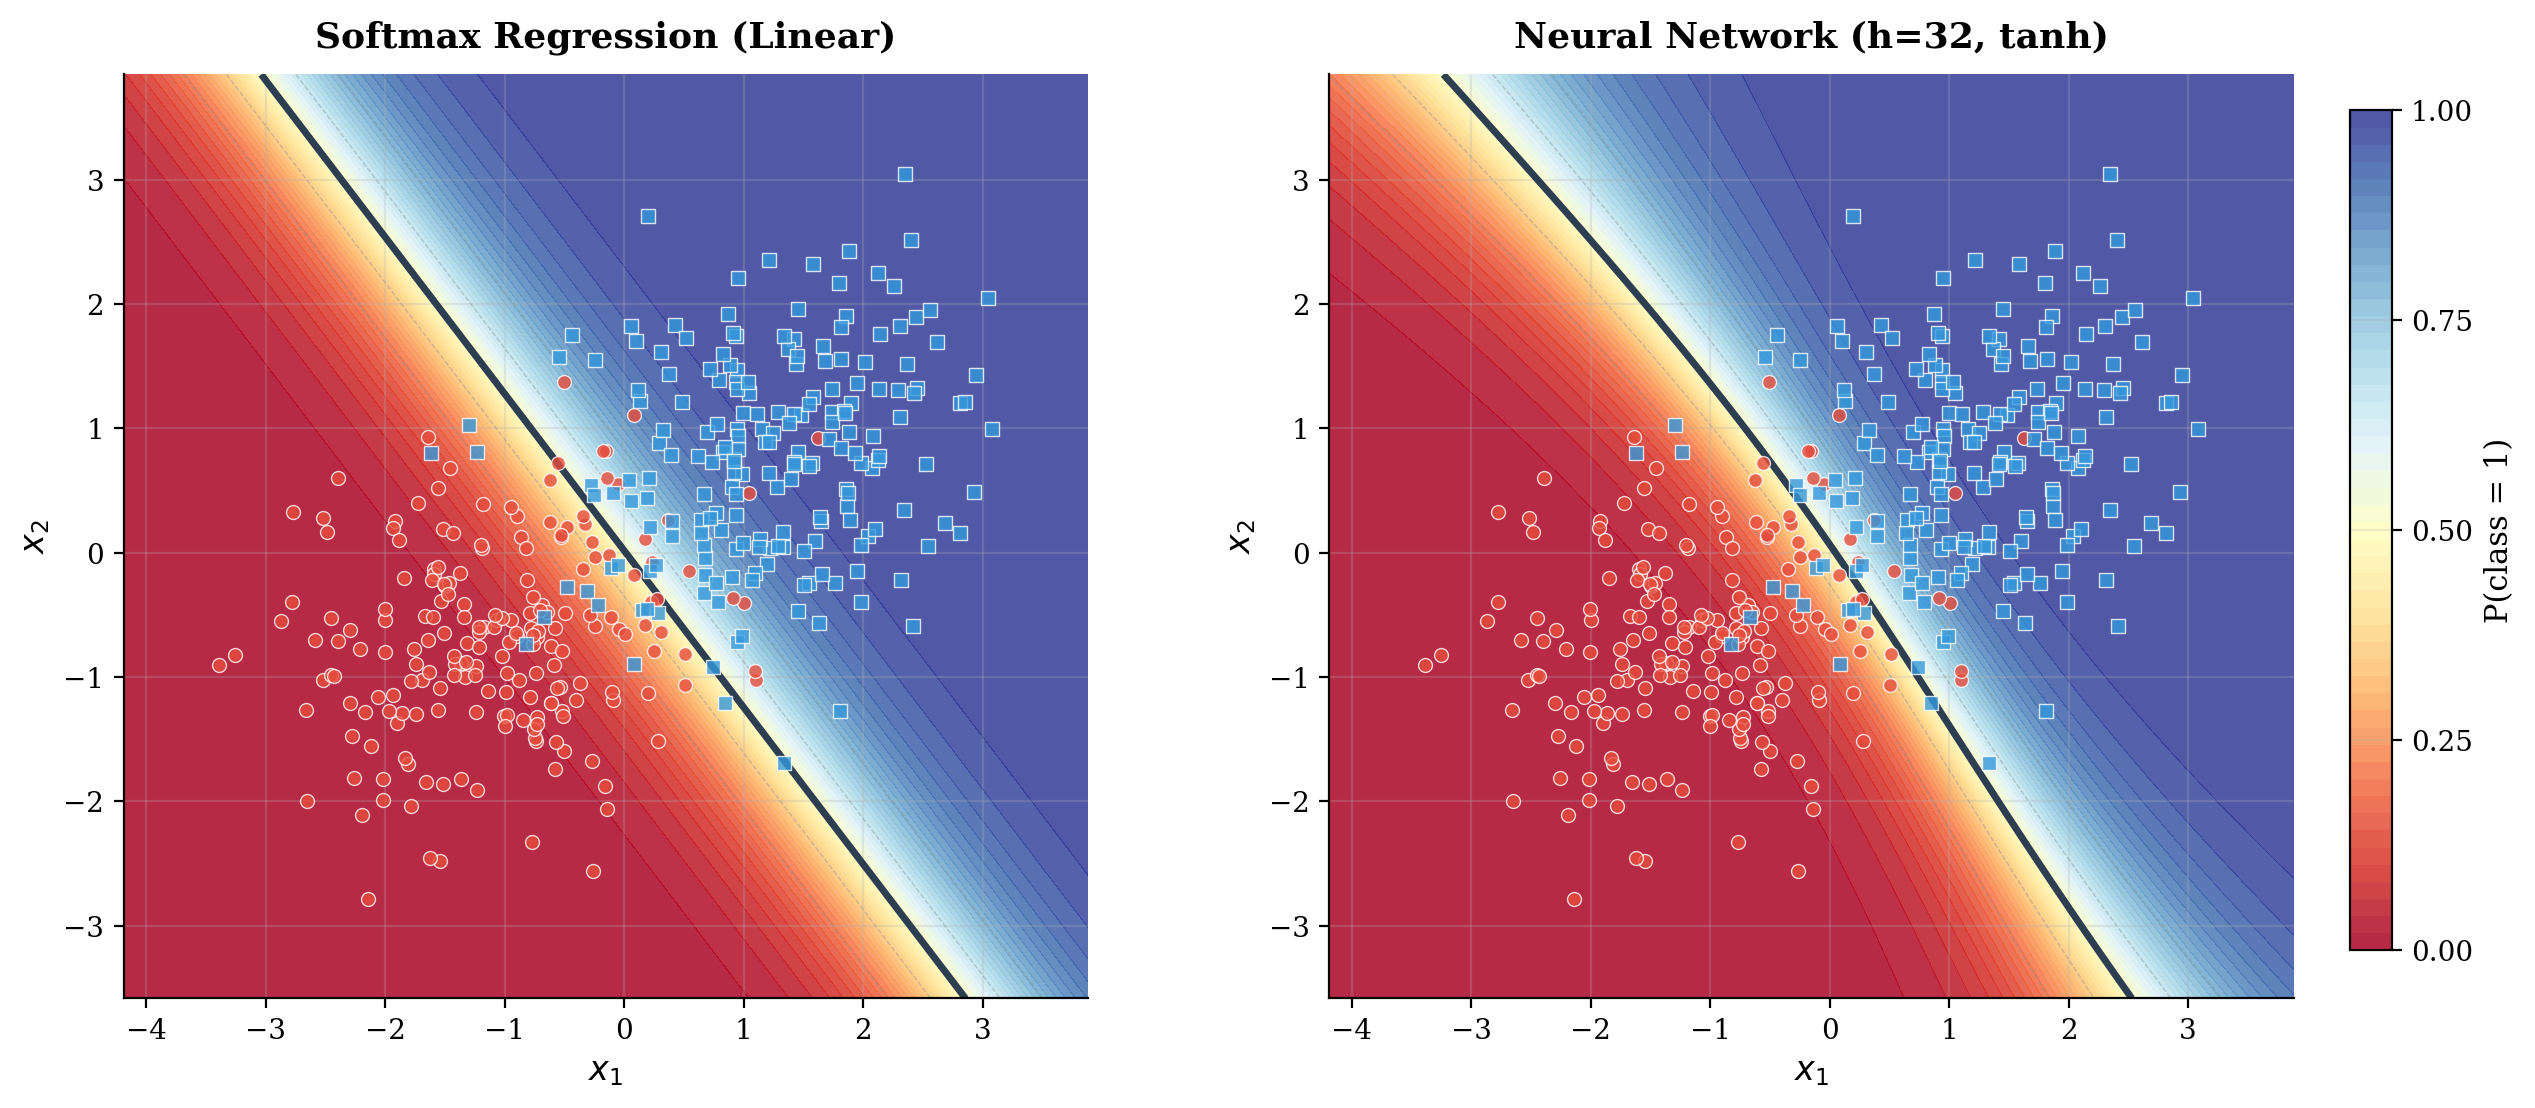
\includegraphics[width=0.65\textwidth]{../figures/comparison_lineargaussian.png}
  \caption{Decision boundaries on the Linear Gaussian task.  Left: Softmax Regression.
           Right: Neural Network ($H{=}32$).  Both produce a near-identical linear
           separator.}
  \label{fig:comparison_gaussian}
\end{figure}

\paragraph{Moons.}
Figure~\ref{fig:comparison_moons} reveals the geometric difference.  Softmax Regression
places a straight line through curved data, failing substantially.  The neural network
maps the original 2-D space into $\R^{32}$ via $\tanh(\bW_1\bx+\bb_1)$, where the arcs
become linearly separable, achieving near-$100\%$ accuracy.

\begin{figure}[H]
  \centering
  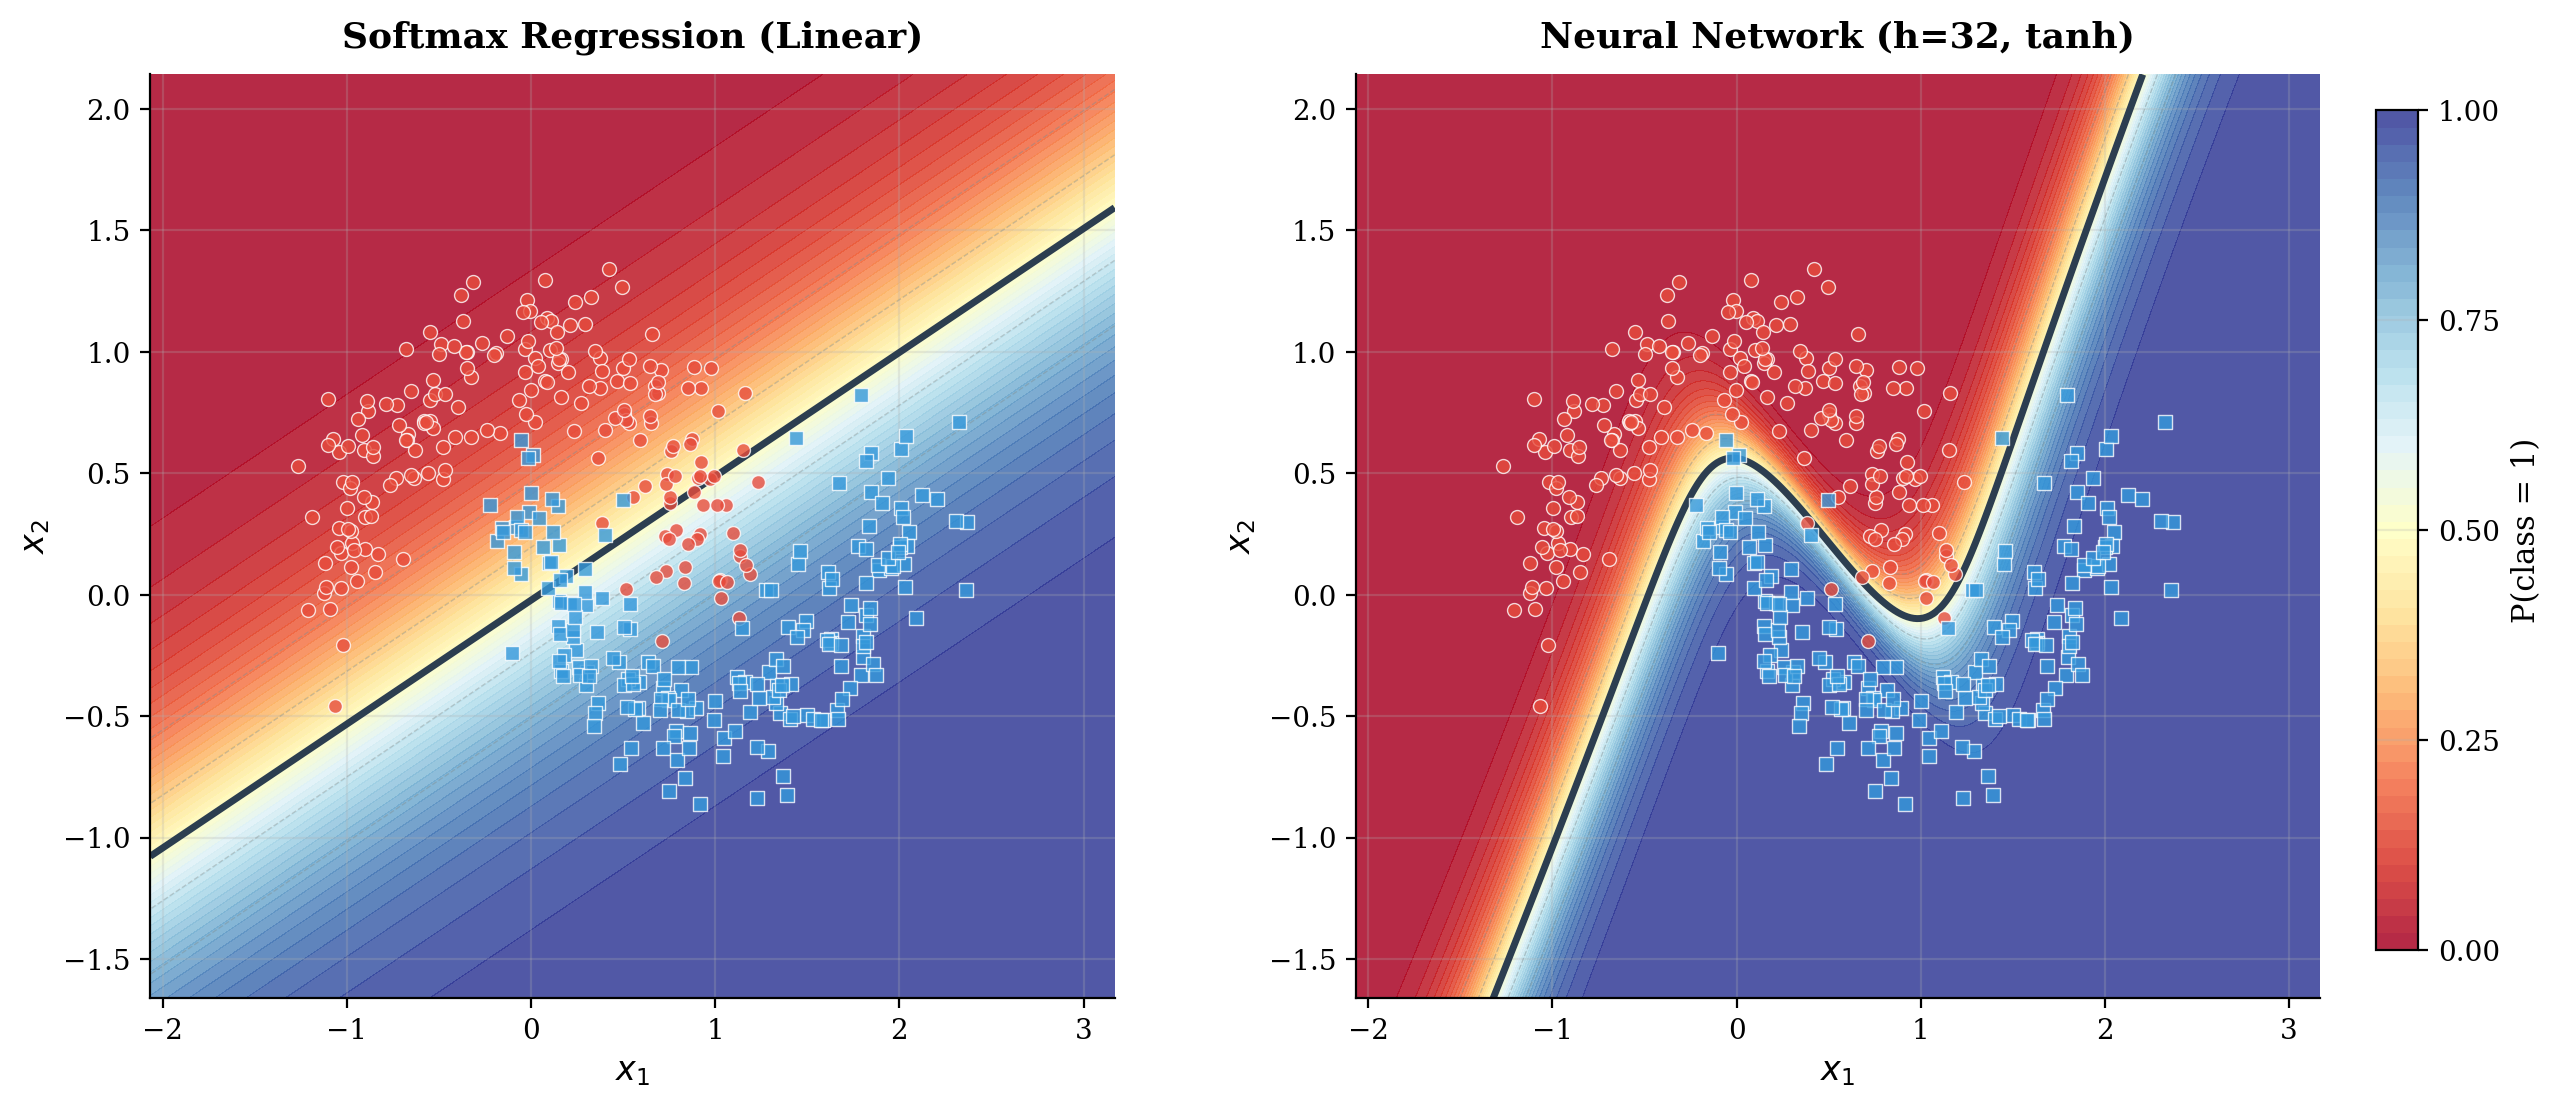
\includegraphics[width=0.65\textwidth]{../figures/comparison_moons.png}
  \caption{Decision boundaries on the Moons task.  Left: Softmax Regression (fails).
           Right: Neural Network ($H{=}32$, succeeds).}
  \label{fig:comparison_moons}
\end{figure}

% ──────────────────────────────────────────────────────────────────
\subsection{Capacity Ablation on Moons}

We trained the neural network on Moons with $H\in\{2,8,32\}$ (Figure~\ref{fig:ablation}):
\begin{itemize}[leftmargin=1.4em,itemsep=0.15em]
  \item $H{=}2$: angular, low-confidence boundaries---too few dimensions.
  \item $H{=}8$: reasonable curved boundary, uneven confidence near the boundary.
  \item $H{=}32$: smooth, high-confidence boundary tightly hugging the data manifold.
\end{itemize}

This demonstrates a monotonic relationship between hidden width and boundary quality
\emph{on this task}, because the intrinsic complexity demands nonlinear expressiveness.
On the Gaussian task, all three widths produce essentially the same linear boundary.

\begin{figure}[H]
  \centering
  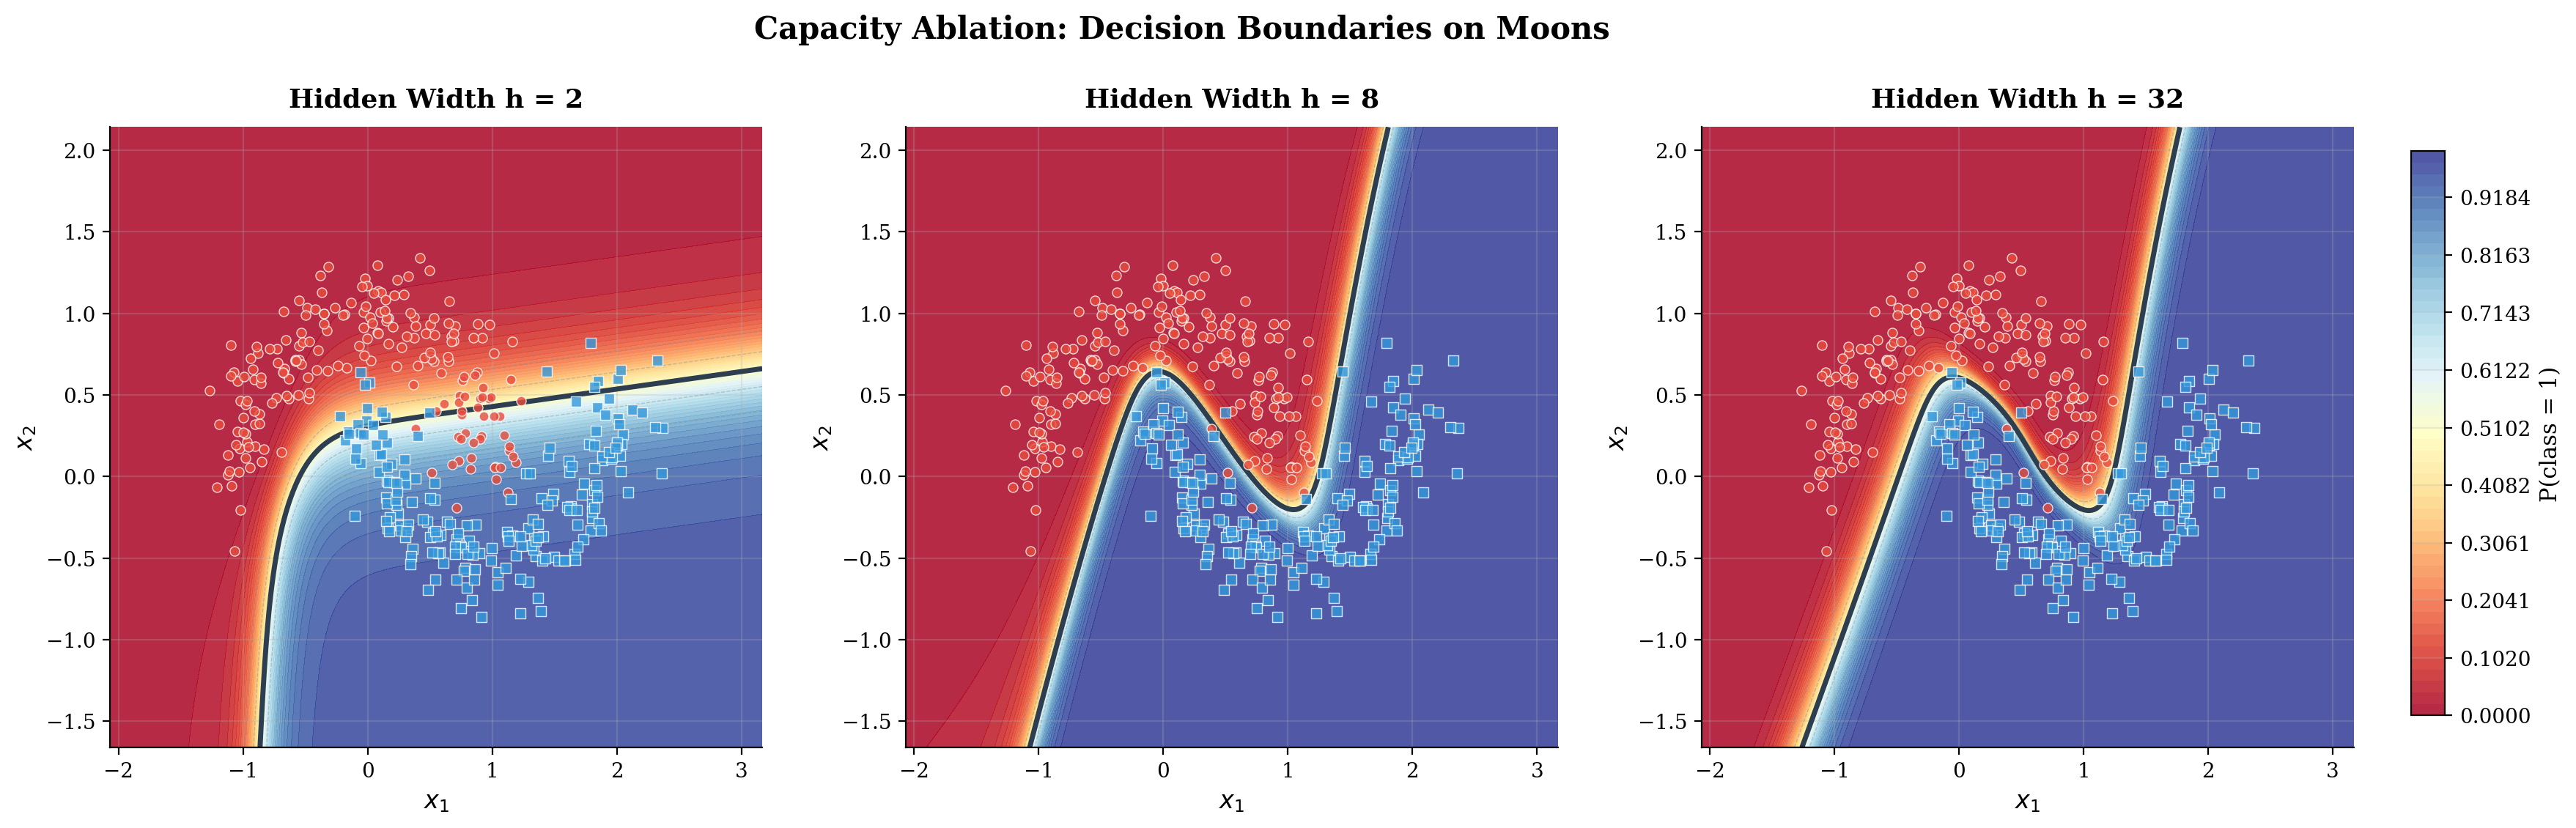
\includegraphics[width=0.95\textwidth]{../figures/capacity_ablation_boundaries.png}
  \caption{Capacity ablation on Moons.  Left to right: $H{=}2$, $H{=}8$, $H{=}32$.}
  \label{fig:ablation}
\end{figure}

% ──────────────────────────────────────────────────────────────────


\subsection{Digits Benchmark}

Table~\ref{tab:digits_main} summarises the core comparison with five-seed evaluation.

\begin{table}[H]
\centering
\caption{Digits benchmark: five-seed summary (mean $\pm$ 95\% CI).}
\label{tab:digits_main}
\begin{tabular}{@{}lcc@{}}
\toprule
\textbf{Model} & \textbf{Test Accuracy} & \textbf{Test Cross-Entropy} \\
\midrule
Softmax Regression & $93.26\%\;\pm\;0.73\%$ & $0.2692\;\pm\;0.0067$ \\
Neural Network ($H{=}32$) & $95.71\%\;\pm\;0.91\%$ & $0.1566\;\pm\;0.0162$ \\
\bottomrule
\end{tabular}
\end{table}

The neural network improves accuracy by ${\sim}2.5$ percentage points and reduces
cross-entropy by ${\sim}42\%$.  The $95\%$ confidence intervals do not overlap.  The CE
reduction is proportionally larger than the accuracy gain, indicating better-calibrated
probabilities.
Figure~\ref{fig:loss_curves_digits} shows representative training dynamics; neither model
exhibits severe overfitting within the 200-epoch budget.

\begin{figure}[H]
  \centering
  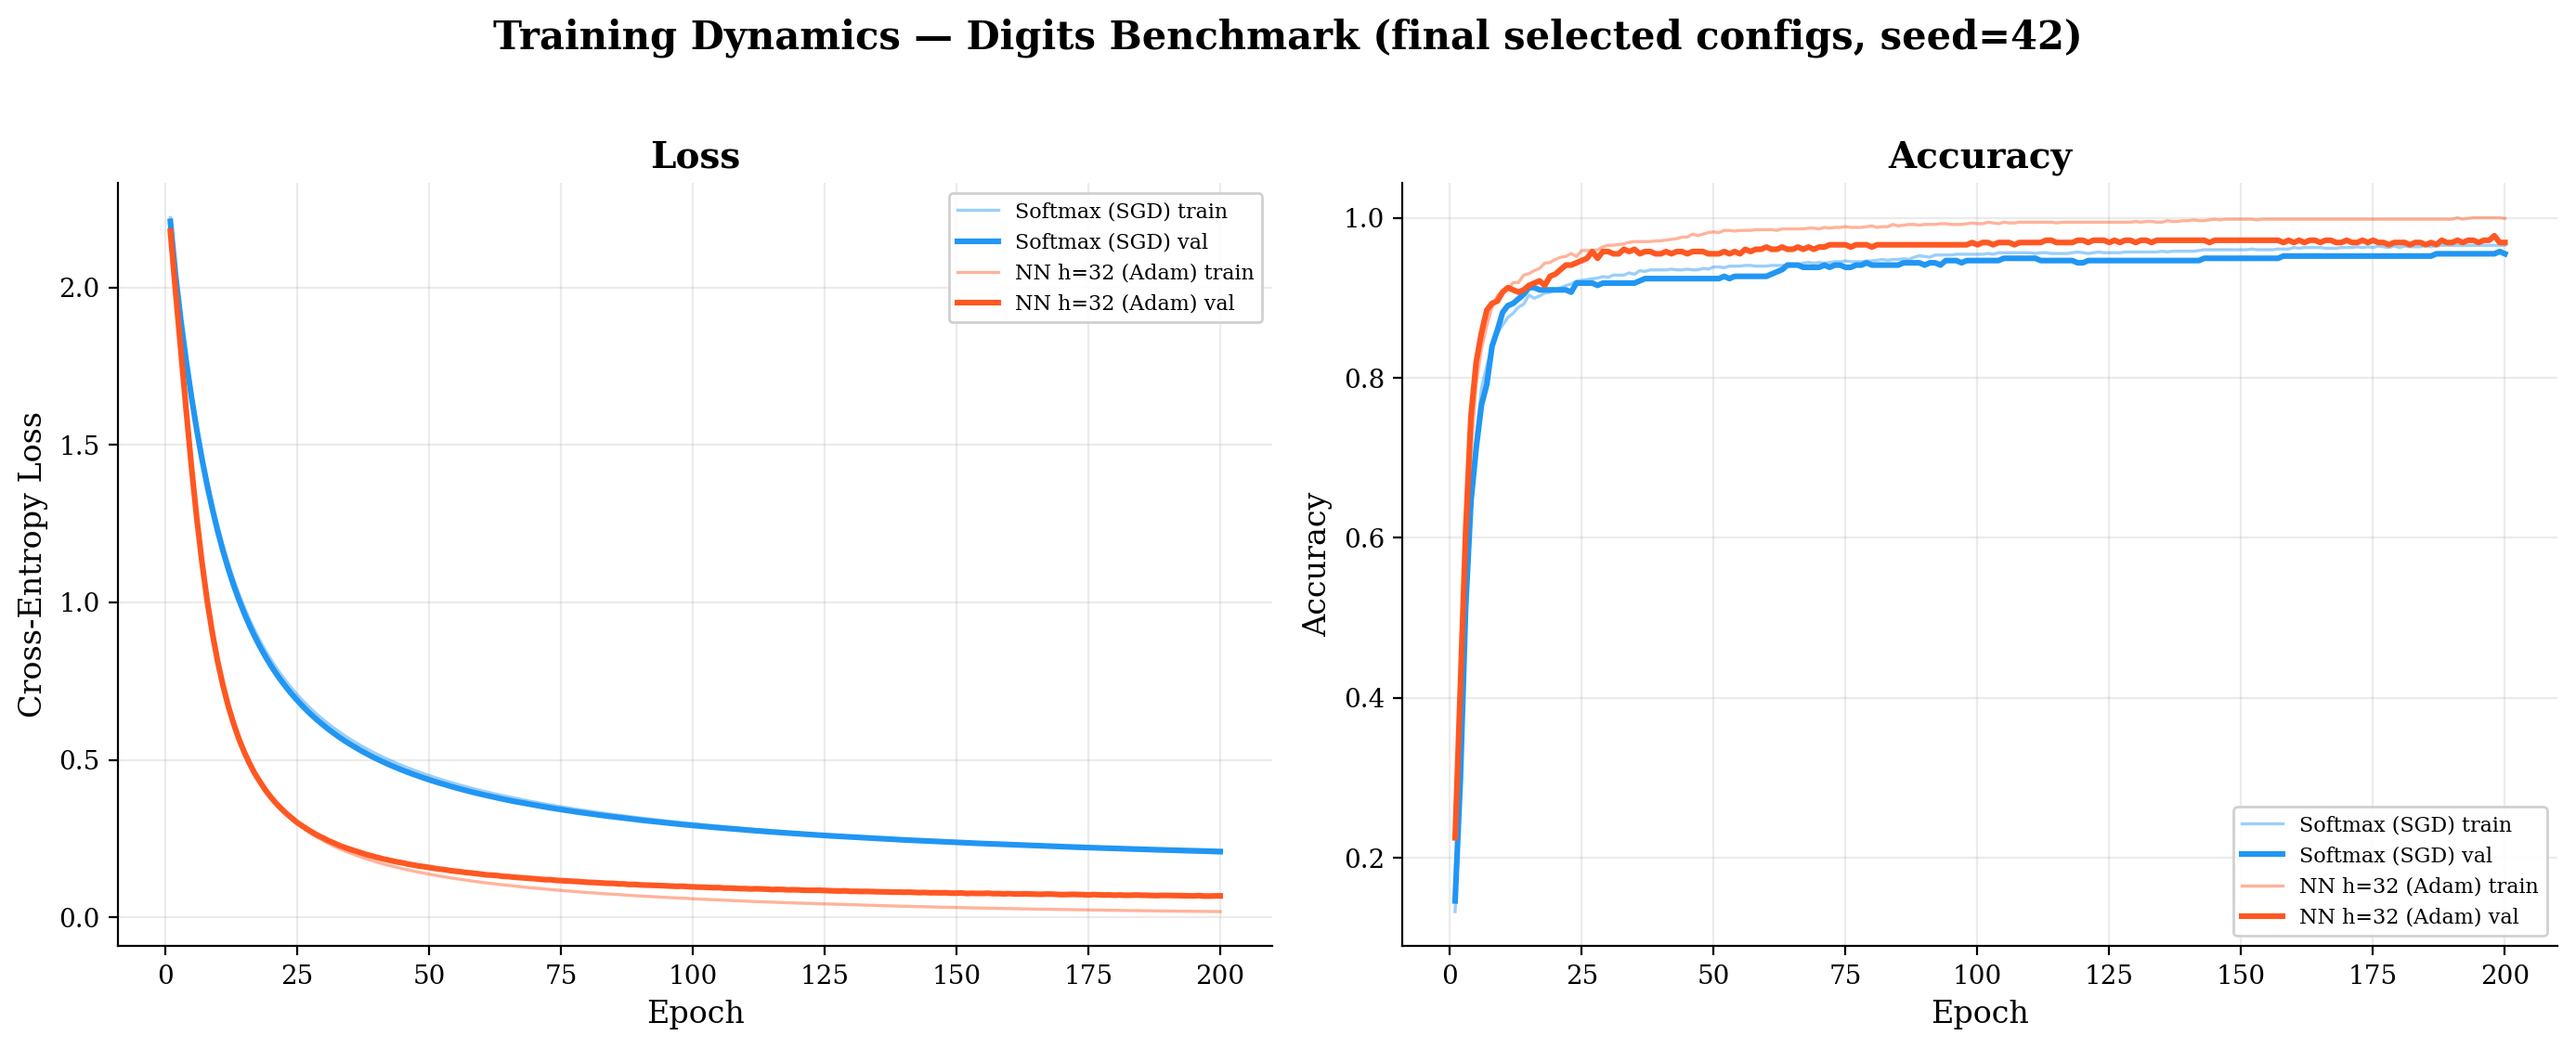
\includegraphics[width=0.75\textwidth]{../figures/loss_curves_digits.png}
  \caption{Training dynamics on the Digits benchmark (single representative seed).}
  \label{fig:loss_curves_digits}
\end{figure}

% ──────────────────────────────────────────────────────────────────
\subsection{Optimizer Study on Digits}
\label{sec:optimizer}

Three optimisers were compared on the neural network ($H{=}32$), shown in
Table~\ref{tab:optimizers} and Figure~\ref{fig:optimizers}.

\begin{table}[H]
\centering
\caption{Optimizer study on Digits (NN, $H{=}32$, best validation checkpoint).}
\label{tab:optimizers}
\begin{tabular}{@{}lccc@{}}
\toprule
\textbf{Optimizer} & \textbf{Test Acc.} & \textbf{Test CE} & \textbf{Best Epoch} \\
\midrule
SGD ($\eta{=}0.05$) & 94.84\% & 0.1700 & 197 \\
Momentum ($\eta{=}0.05,\;\mu{=}0.9$) & 95.38\% & 0.1653 & 197 \\
Adam ($\eta{=}0.001$) & 95.11\% & 0.1507 & 197 \\
\bottomrule
\end{tabular}
\end{table}

Adam and Momentum converge to low validation loss faster than plain SGD, but all three
reach comparable final accuracy.  Adam achieves the lowest CE ($0.1507$), suggesting better
calibration, while Momentum yields the highest accuracy ($95.38\%$).  The practical
conclusion: for this task, optimiser choice has a secondary effect (${\sim}0.5$~ppt spread)
relative to model-class choice (${\sim}2.5$~ppt gap).

\begin{figure}[H]
  \centering
  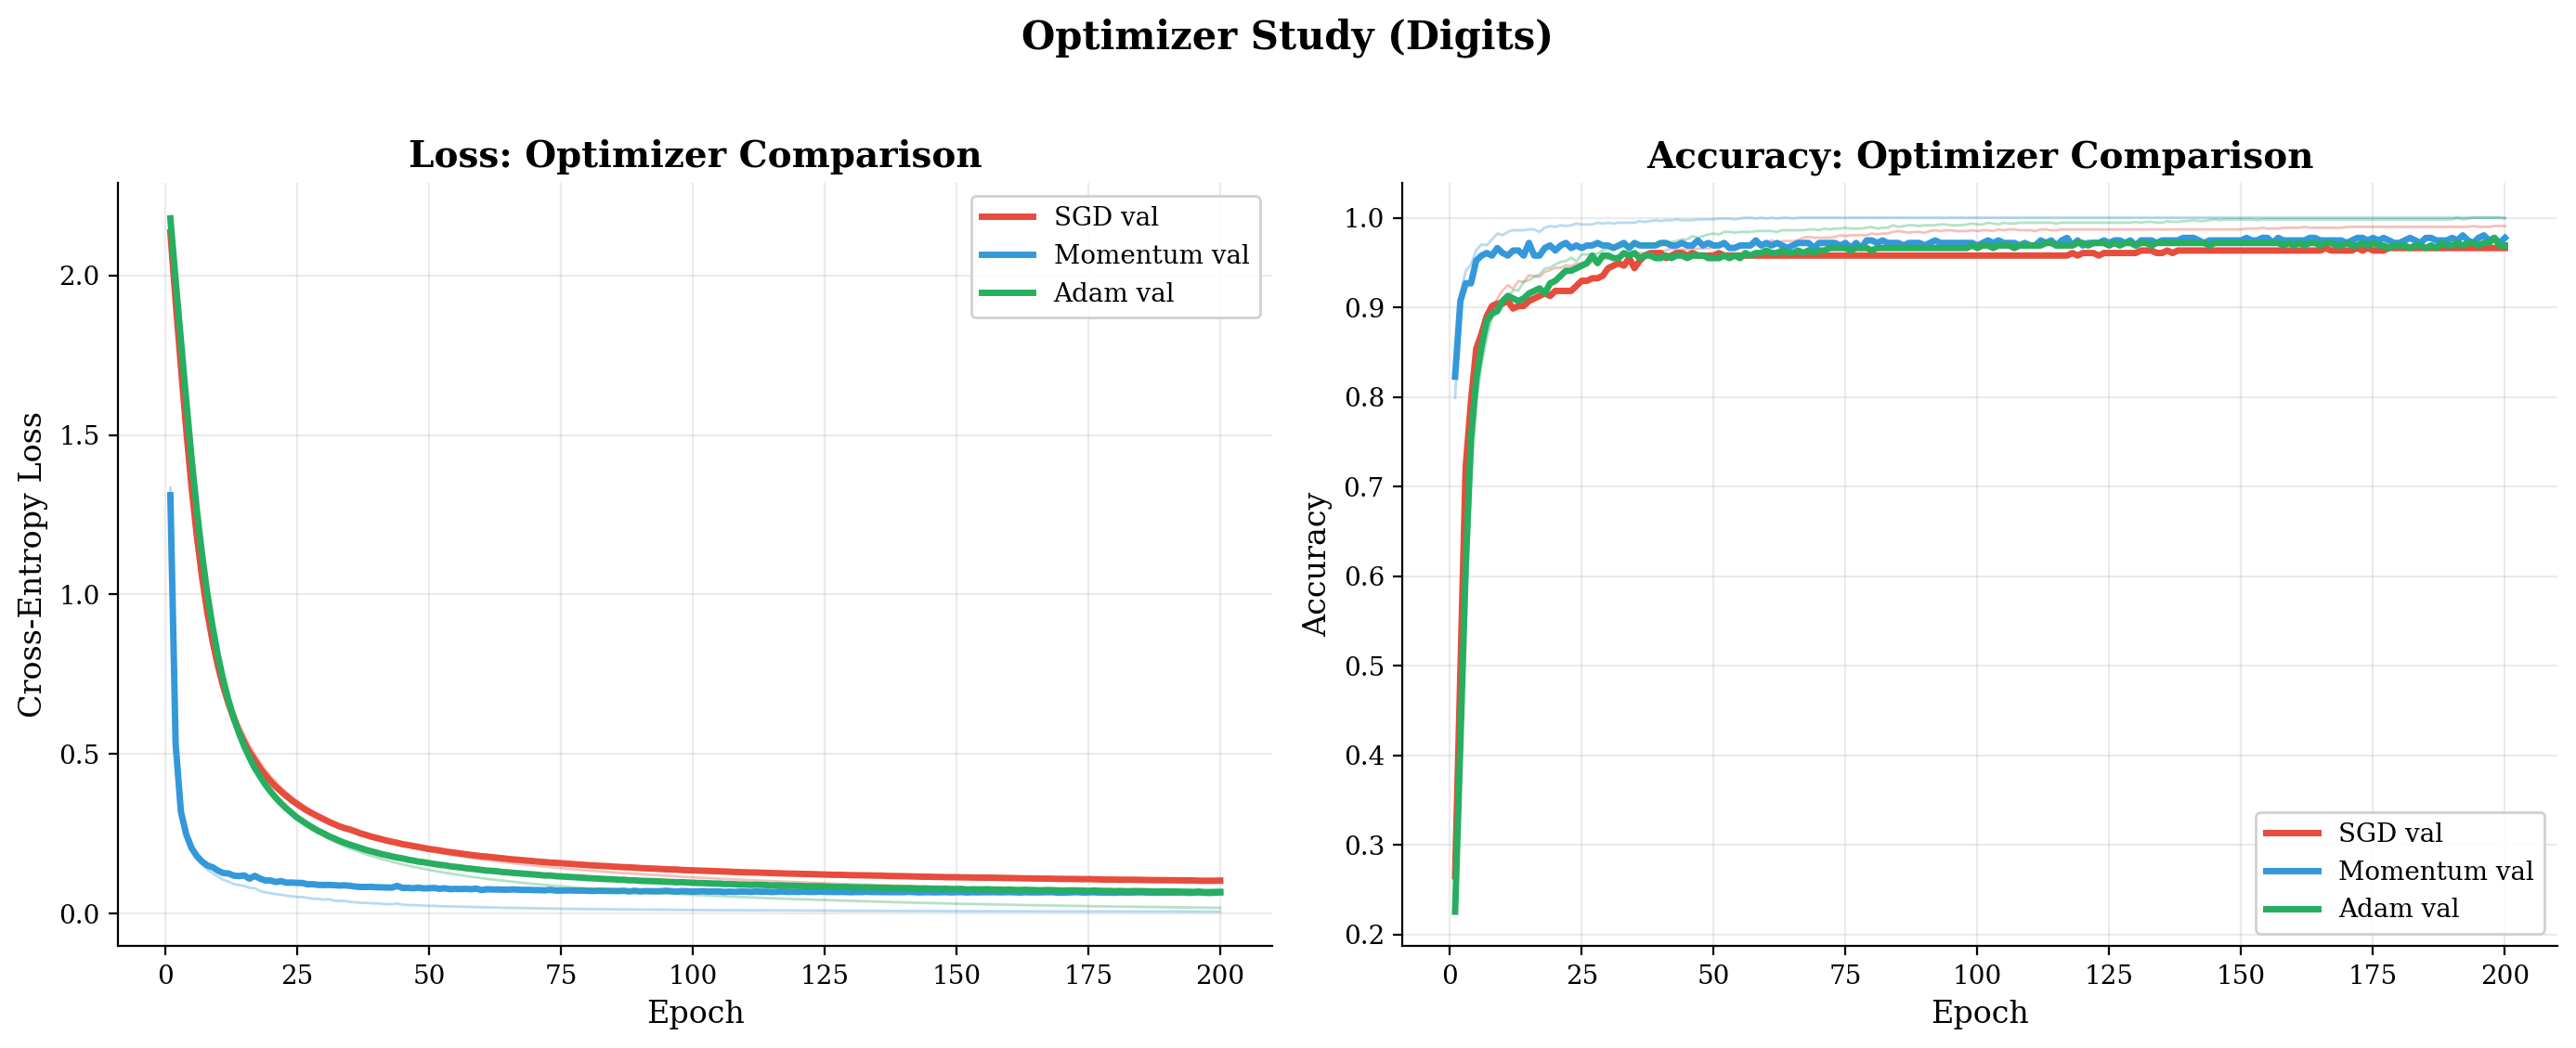
\includegraphics[width=0.85\textwidth]{../figures/optimizer_study_digits.png}
  \caption{Validation loss and accuracy across optimisers (NN, $H{=}32$, Digits).}
  \label{fig:optimizers}
\end{figure}

% ──────────────────────────────────────────────────────────────────
\subsection{Failure-Case Analysis: Under-Capacity Bottleneck ($H{=}2$)}
\label{sec:failure}

We deliberately trained a neural network with $H{=}2$ on the 10-class Digits task.  The
hidden layer projects the 64-dimensional input to a 2-dimensional representation via
$\bh = \tanh(\bW_1\bx + \bb_1) \in [-1,1]^2$ before the output layer attempts to
classify into 10~classes.

\begin{table}[H]
\centering
\caption{Failure case: $H{=}2$ bottleneck on Digits.}
\label{tab:failure}
\begin{tabular}{@{}lcc@{}}
\toprule
\textbf{Model} & \textbf{Test Accuracy} & \textbf{Test Cross-Entropy} \\
\midrule
Softmax Regression (linear) & 93.26\% & 0.2692 \\
NN ($H{=}2$) & 58.97\% & 1.1133 \\
NN ($H{=}32$) & 95.71\% & 0.1566 \\
\bottomrule
\end{tabular}
\end{table}

The $H{=}2$ model achieves only $58.97\%$ accuracy---far below even the linear baseline
($93.26\%$).  This is a striking result: a nonlinear model with a hidden layer performs
\emph{worse} than a linear model without one.

\paragraph{Why it fails: a geometric argument.}
The failure is \emph{representational}, not optimisational.  With $H{=}2$, the hidden
layer maps $\R^{64}$ to $[-1,1]^2$.  The output layer then has access to only a
2-dimensional input from which it must carve out 10 linearly separable regions.  In
$\R^2$, the maximum number of regions that $K$ hyperplanes can create is
$\binom{K}{0}+\binom{K}{1}+\binom{K}{2}$, but separating 10 classes into distinct convex
regions with only 2-D linear boundaries is geometrically impossible unless the hidden
representation arranges all 10 classes into perfectly separable clusters---which two
coordinates cannot achieve for the complexity of handwritten digits.

% The optimiser faithfully minimises the loss \emph{within} the representational constraints
% of the architecture, but the global minimum of the $H{=}2$ loss surface itself corresponds
% to a poor classifier.  Despite using the same optimiser, learning rate, epoch budget, and
% regularisation that yield $95.71\%$ with $H{=}32$, the bottleneck architecture stalls at
% $58.97\%$.  Both training and validation loss remain high throughout (Figure~\ref{fig:failure}).

\paragraph{The lesson.}
\textbf{Representational capacity must match task complexity before optimisation can be
effective.}  Increasing $H$ from 2 to 32 does not change the optimiser---it changes the
\emph{geometry of the function class}, enabling richer internal representations.  This
failure case also explains why adding a hidden layer is not inherently beneficial: if the
width is insufficient, the bottleneck can actually \emph{destroy} information present in
the original input, making the nonlinear model worse than the linear baseline that
preserves all $d$ dimensions.

\begin{figure}[H]
  \centering
  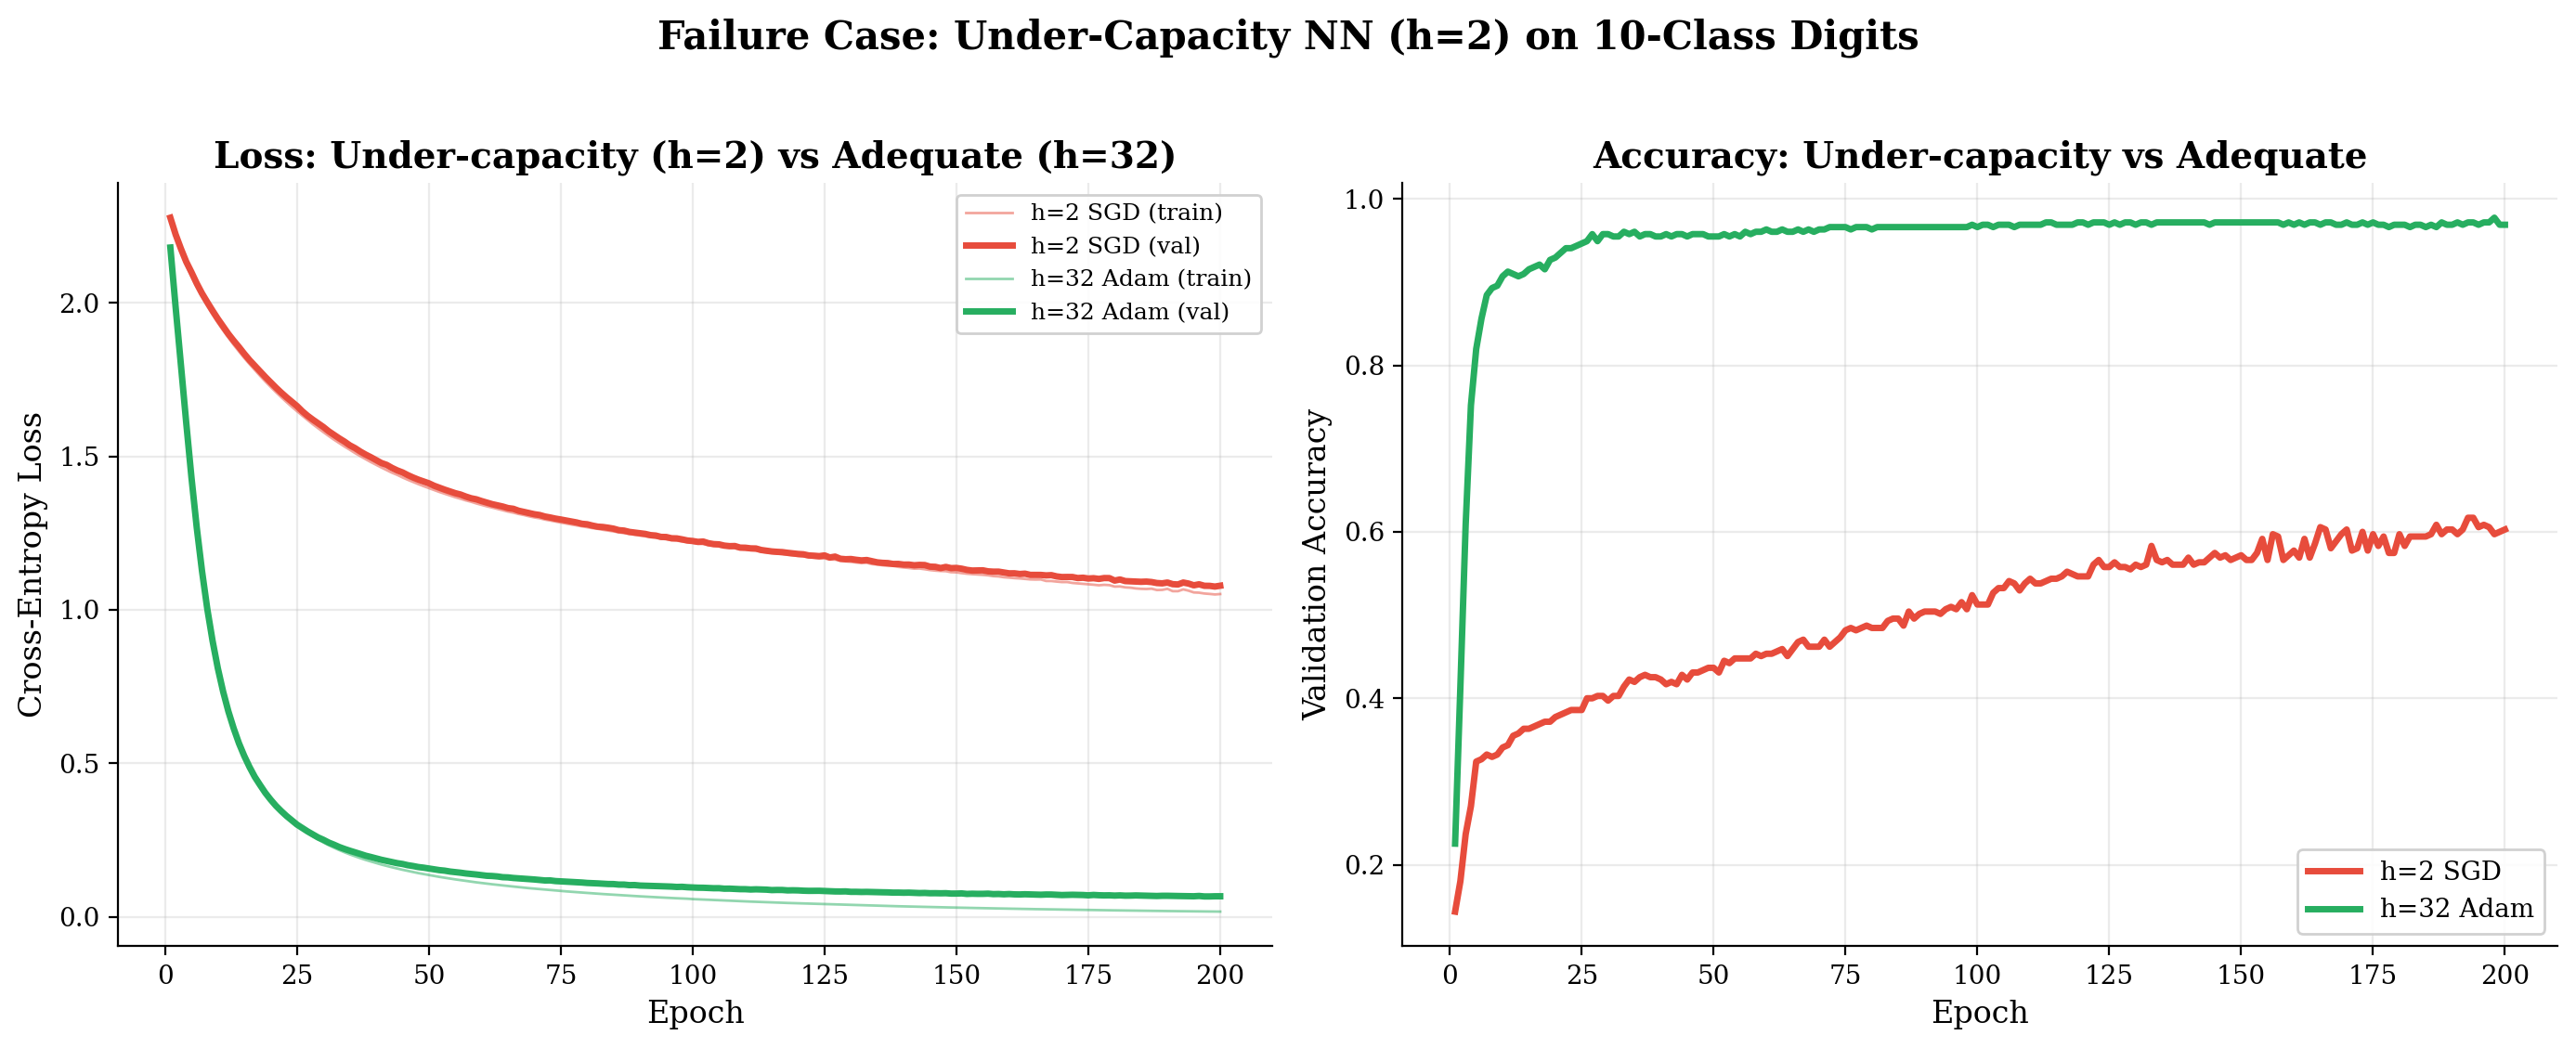
\includegraphics[width=0.85\textwidth]{../figures/failure_analysis.png}
  \caption{Failure case.  The $H{=}2$ bottleneck (red) severely underfits with high
           residual loss, while the $H{=}32$ model (green) converges to low loss.  The
           gap is due to representational capacity, not optimisation quality.}
  \label{fig:failure}
\end{figure}

% \subsection{Failure-Case Analysis: Under-Capacity Bottleneck ($H{=}2$)}
% \label{sec:failure}

% We deliberately trained a network with $H{=}2$ on 10-class Digits.  The hidden layer
% compresses 64 dimensions to $[-1,1]^2$ before attempting 10-class classification.

% \begin{table}[H]
% \centering
% \caption{Failure case: $H{=}2$ bottleneck on Digits.}
% \label{tab:failure}
% \begin{tabular}{@{}lcc@{}}
% \toprule
% \textbf{Model} & \textbf{Test Accuracy} & \textbf{Test Cross-Entropy} \\
% \midrule
% Softmax Regression (linear) & 93.26\% & 0.2692 \\
% NN ($H{=}2$) & 58.97\% & 1.1133 \\
% NN ($H{=}32$) & 95.71\% & 0.1566 \\
% \bottomrule
% \end{tabular}
% \end{table}

% The $H{=}2$ model achieves only $58.97\%$---far below even the linear baseline.  A nonlinear
% model \emph{worse} than a linear one.

% \paragraph{Why it fails: a geometric argument.}
% The failure is \emph{representational}, not optimisational.  With $H{=}2$, the network maps
% $\R^{64}$ to $[-1,1]^2$.  The output layer has only 2~dimensions from which to carve 10
% regions---geometrically impossible for complex digit structure.  The optimiser faithfully
% minimises the loss within the architecture's constraints, but the global minimum itself
% corresponds to a poor classifier.  Both training and validation loss remain high
% (Figure~\ref{fig:failure}), confirming \emph{underfitting} due to capacity, not optimisation.

% \textbf{Lesson:} Representational capacity must match task complexity before optimisation can
% be effective.  Increasing $H$ from 2 to 32 expands the hypothesis class, enabling richer
% representations.  An insufficient bottleneck can \emph{destroy} information present in the
% original input, making the nonlinear model worse than the linear baseline.

% \begin{figure}[H]
%   \centering
%   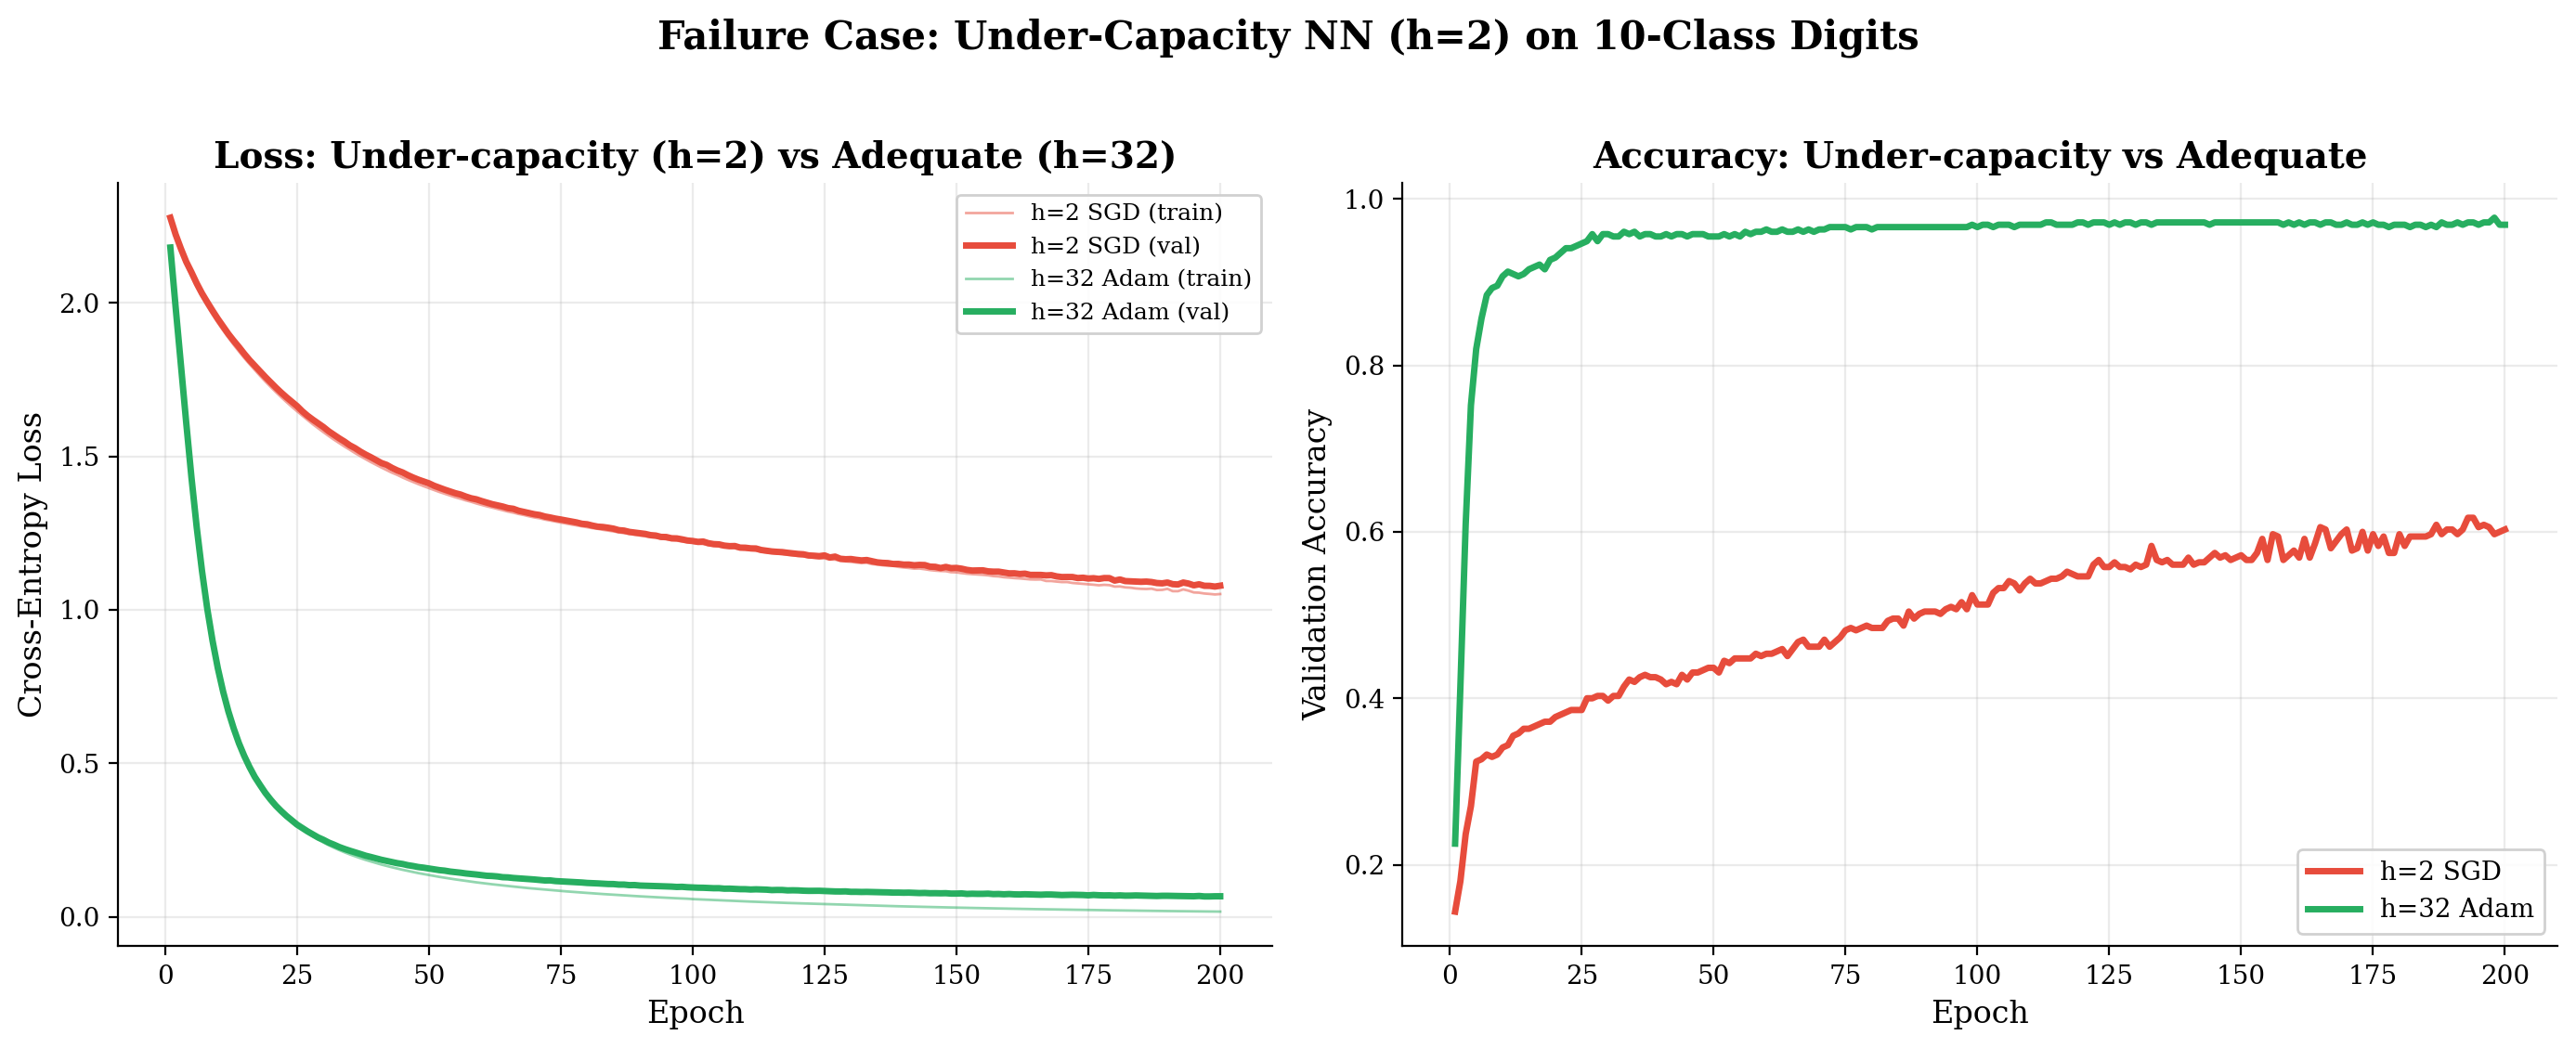
\includegraphics[width=0.85\textwidth]{../figures/failure_analysis.png}
%   \caption{Failure case.  $H{=}2$ (red) underfits with high residual loss; $H{=}32$
%            (green) converges to low loss.}
%   \label{fig:failure}
% \end{figure}

% ================================================================
\section{Advanced Track A: PCA/SVD and Input Geometry}
\label{sec:pca}
% ================================================================

We computed the SVD of the mean-centred training matrix
$\bX_c = \bX - \bone\bar{\bx}^\top = \mathbf{U}\mathbf{\Sigma}\mathbf{V}^\top$
to study the linear structure before any learning occurs.

\paragraph{Scree analysis.}
Figure~\ref{fig:pca_scree} shows rapid singular-value decay:

\begin{center}
\begin{tabular}{@{}lcccc@{}}
\toprule
Components $m$ & 5 & 10 & 20 & 40 \\
\midrule
Cumulative variance & 54.7\% & 74.1\% & 89.6\% & 98.9\% \\
\bottomrule
\end{tabular}
\end{center}

\noindent
The top 20 components capture $89.6\%$ of total variance; the remaining 44~dimensions
contribute noise-level variance, indicating substantial low-dimensional structure.

\paragraph{2-D projection.}
Figure~\ref{fig:pca_2d} shows digits projected onto the first two PCs.  Digits 0 and 6
form distinct clusters; digits 3, 5, and 8 overlap (shared curved strokes).  Two dimensions
are insufficient for full separation but reveal meaningful coarse structure.

\paragraph{Classification at reduced dimensions.}
Table~\ref{tab:pca} shows Softmax accuracy on PCA-compressed inputs:

\begin{table}[H]
\centering
\caption{Softmax Regression accuracy on PCA-reduced Digits inputs.}
\label{tab:pca}
\begin{tabular}{@{}lcccc@{}}
\toprule
$m$ & 10 & 20 & 40 & 64 (full) \\
\midrule
Val.\ Accuracy & 92.68\% & 94.08\% & 94.93\% & 95.49\% \\
Val.\ CE Loss  & 0.2874  & 0.2292  & 0.2133  & 0.2109  \\
\bottomrule
\end{tabular}
\end{table}

At $m{=}20$, Softmax still achieves $94.08\%$---only $1.4$ points below the full result.
This reveals \textbf{substantial linear structure} in the input space.  The neural network's
${\sim}2.5$-point advantage comes from exploiting \emph{residual nonlinear} interactions that
PCA---a purely linear projection---cannot recover.

\begin{figure}[H]
  \centering
  \begin{subfigure}[b]{0.50\linewidth}
    \centering
    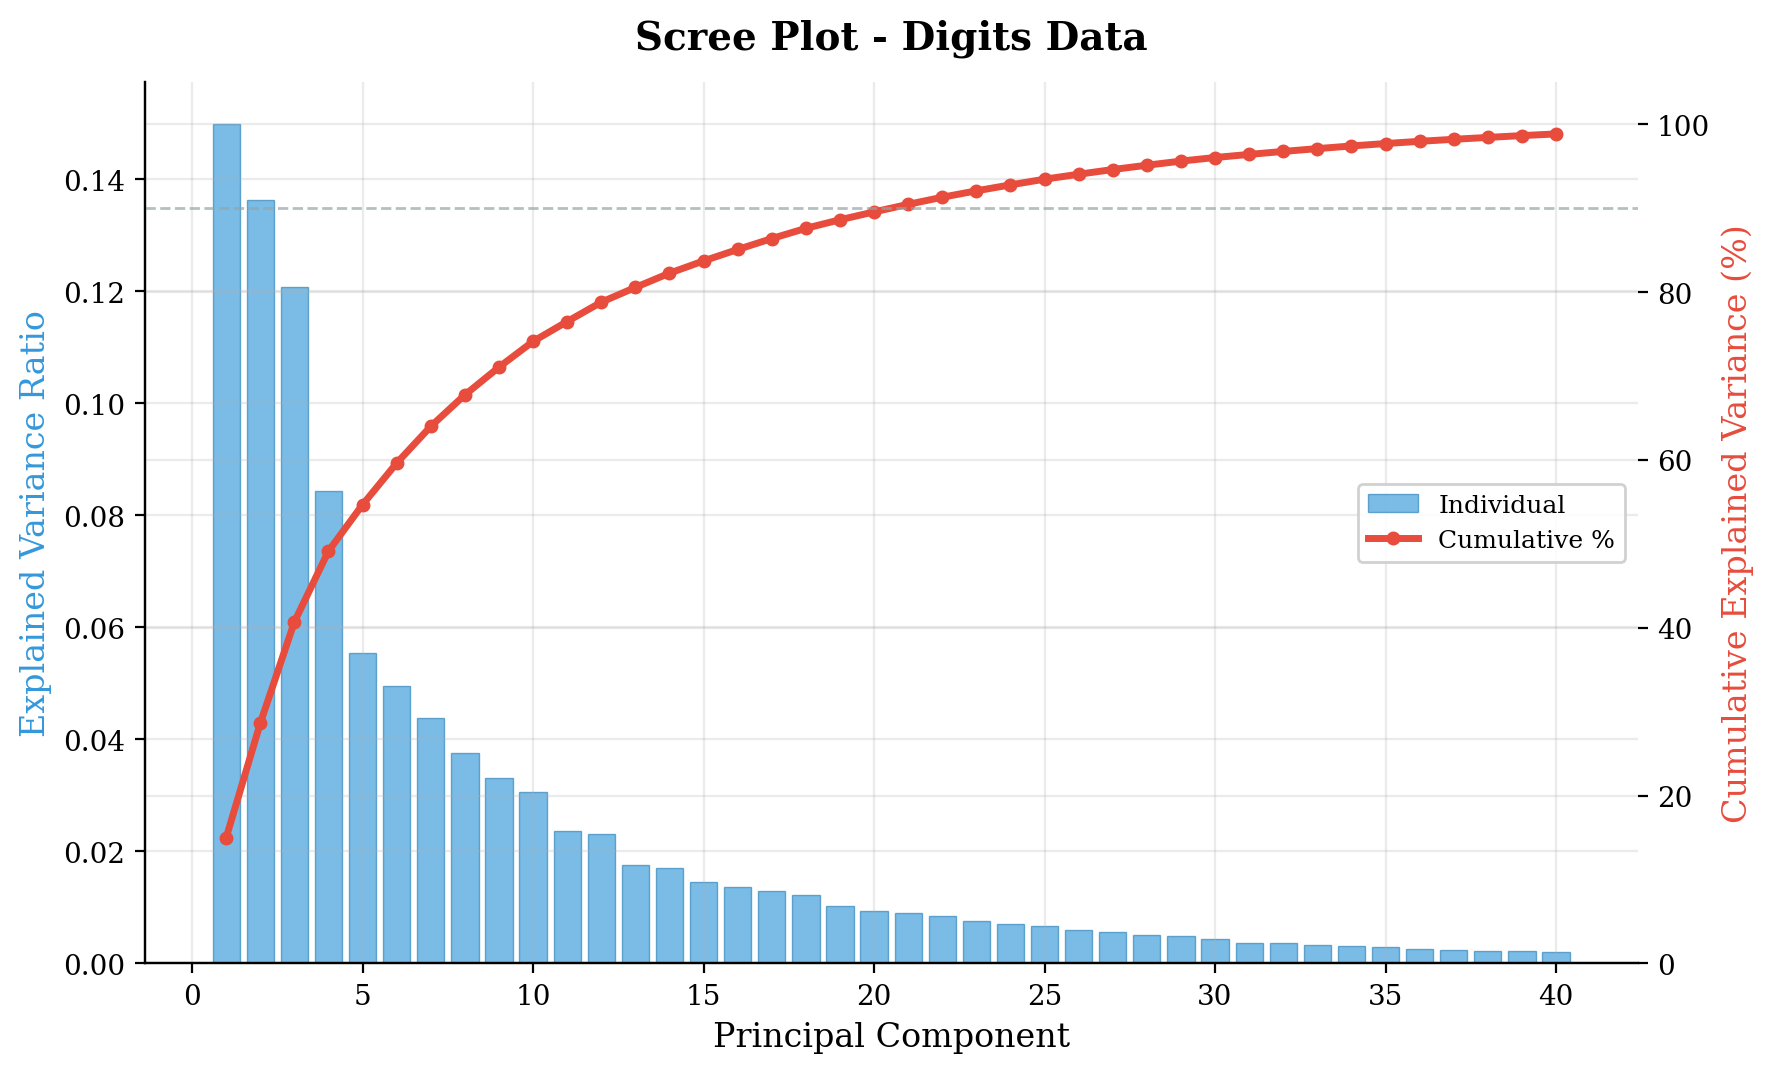
\includegraphics[width=\textwidth]{../figures/pca_scree_digits.png}
    \caption{Scree plot and cumulative explained variance.}
    \label{fig:pca_scree}
  \end{subfigure}\hfill
  \begin{subfigure}[b]{0.48\linewidth}
    \centering
    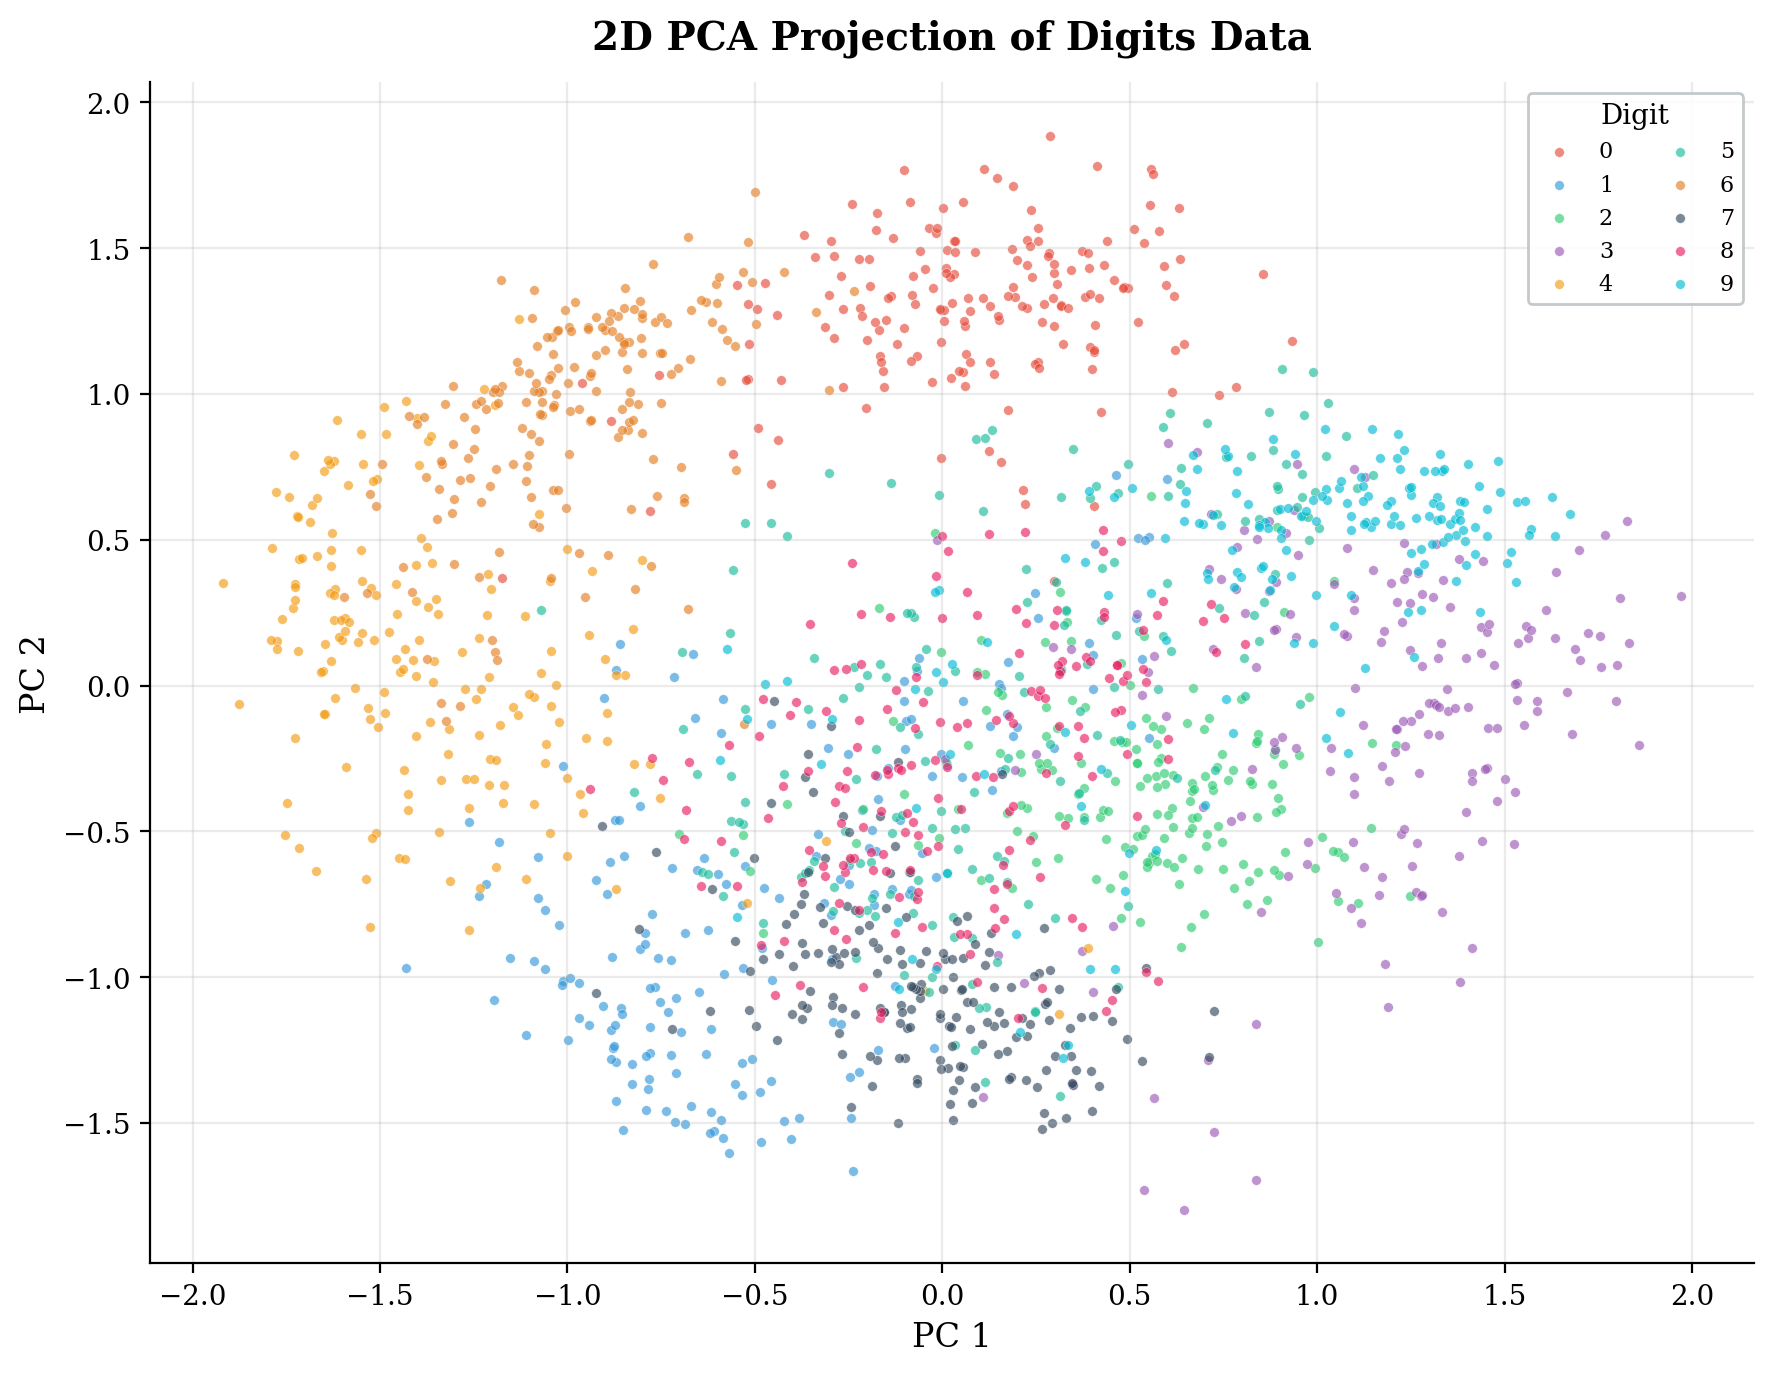
\includegraphics[width=\textwidth]{../figures/pca_2d_digits.png}
    \caption{2-D PCA projection of Digits classes.}
    \label{fig:pca_2d}
  \end{subfigure}
  \caption{Track A: PCA/SVD analysis of the Digits dataset.}
  \label{fig:pca}
\end{figure}

% ================================================================
\section{Discussion: Interpretive Analysis}
\label{sec:discussion}
% ================================================================

We answer the five core interpretive questions, drawing exclusively on the evidence above.

\begin{enumerate}[leftmargin=2em,itemsep=0.5em]

\item \textbf{When is the linear model geometrically sufficient, and when is it not?}

The linear model suffices when the Bayes-optimal boundary is a hyperplane.  This holds
rigorously for the Gaussian task (Equation~\ref{eq:logodds}) and approximately for Digits,
where Softmax reaches $93.26\%$ and PCA confirms that dominant discriminative directions
are linear.  The linear model is \emph{insufficient} on Moons, where no affine function
separates the arcs (Figure~\ref{fig:comparison_moons}).

\item \textbf{What representational change does the hidden layer provide?}

The map $\bh = \tanh(\bW_1\bx+\bb_1)$ is a learned nonlinear coordinate change from
$\R^d$ to $\R^H$.  On Moons, it ``untwists'' the arcs into linearly separable clusters
in $\R^{32}$.  On Digits, it captures nonlinear feature combinations (stroke curvatures,
junctions) that linear projections cannot, accounting for the ${\sim}2.5$-point gain.  The
PCA comparison confirms this gain is from \emph{nonlinear} structure.

\item \textbf{When does additional model complexity fail to justify itself?}

\emph{(a)} When the baseline captures the geometry: on Gaussian, the NN matches Softmax
with $3.7{\times}$ more parameters.  \emph{(b)} When complexity is of the wrong kind:
Softmax at $m{=}20$ PCA dimensions ($94.08\%$) is within $1.6$ points of the full NN
($95.71\%$).  If the engineering cost is high and the gap is tolerable, the simpler model
may be preferable.

\item \textbf{What does your failure case teach about optimisation, capacity, or
generalisation?}

The $H{=}2$ bottleneck teaches that \emph{capacity is a prerequisite optimisation cannot
substitute}.  Identical optimiser settings yield $58.97\%$ ($H{=}2$) versus $95.71\%$
($H{=}32$).  This distinguishes three failure modes:
\begin{itemize}[leftmargin=1.4em,itemsep=0.1em]
  \item \emph{Optimisation failure}: architecture can represent a solution, optimiser can't
        find it.
  \item \emph{Capacity failure}: architecture \emph{cannot} represent a solution.  $\leftarrow$ this case.
  \item \emph{Generalisation failure}: model fits training but not test data.
\end{itemize}
The $H{=}2$ case is pure capacity failure: increasing $H$ expands the hypothesis class,
not the optimiser.

\item \textbf{What do repeated-seed statistics add beyond a single run?}

A single run depends on random initialisation and mini-batch order.  Five seeds with
$\bar{x}\pm 2.776 \cdot s/\!\sqrt{5}$ bound \emph{expected} performance.  Tight intervals
(Softmax: $\pm 0.73\%$; NN: $\pm 0.91\%$) confirm the ${\sim}2.5$-point gap is robust,
not from one lucky seed.  The NN's wider interval reflects more initialisation sensitivity
from additional parameters.

\end{enumerate}

% ================================================================
\section{Limitations}
\label{sec:limitations}
% ================================================================

\begin{enumerate}[leftmargin=2em,itemsep=0.2em]
  \item \textbf{Architectural scope.}
        Single hidden layer, $\tanh$ only, $H\leq 32$.  Conclusions do not extend to
        deeper networks, wider layers, or alternative activations (ReLU, GELU).

  \item \textbf{Dataset scale and splits.}
        Digits has $d{=}64$, $K{=}10$, ${\sim}1{,}800$ samples with a single fixed split.
        Results may not generalise to high-resolution images, larger class counts, or
        cross-validated protocols.

  \item \textbf{Optimiser and regularisation exploration.}
        Each optimiser was tested at one fixed learning rate; only $L_2$
        ($\lambda{=}10^{-4}$) regularisation was used.  Different schedules, dropout,
        or batch normalisation could change the relative rankings.

  \item \textbf{Repeated-seed sample size.}
        Five seeds assume approximate normality of the accuracy distribution, which
        is difficult to verify with $n{=}5$.

  \item \textbf{Synthetic task simplicity.}
        2-D, 400~points, noise-free labels---illustrative of geometric principles but
        not representative of real-world data ambiguity.  No formal calibration
        analysis (reliability diagrams, ECE) was performed.
\end{enumerate}

Our findings reliably characterise the specific comparison on these three tasks under
this fixed protocol.  They should not be overgeneralised to deeper architectures, larger
datasets, or more sophisticated training pipelines.


\newpage
% ================================================================
% Removed newpage to save space
\section*{References}
% ================================================================
\begin{enumerate}[label={[\arabic*]},leftmargin=2em,itemsep=0.2em]
  \item Deisenroth,~M.\,P., Faisal,~A.\,A., \& Ong,~C.\,S.\ (2020). \textit{Mathematics
        for Machine Learning}. Cambridge University Press.
  \item Murphy,~K.\,P.\ (2022). \textit{Probabilistic Machine Learning: An Introduction}.
        MIT Press.
  \item Goodfellow,~I., Bengio,~Y., \& Courville,~A.\ (2016). \textit{Deep Learning}. MIT
        Press.
  \item Ng,~A.\ \& Katanforoosh,~K. \textit{CS229 Lecture Notes: Deep Learning}. Stanford
        University.  Available at \url{https://cs229.stanford.edu/}.
  \item Stanford CS231n staff. \textit{Neural Networks Part 1: Setting up the Architecture}.
        \url{https://cs231n.github.io/neural-networks-1/}
  \item Stanford CS231n staff. \textit{Optimization Part 2: Backpropagation, Intuitions}.
        \url{https://cs231n.github.io/optimization-2/}
  \item ETH Zurich Learning and Adaptive Systems Group. \textit{Introduction to Machine
        Learning Course Notes}.
        \url{https://las.inf.ethz.ch/teaching/introml-s24}
  \item GitHub. \textit{GitHub Flow}.
        \url{https://docs.github.com/en/get-started/using-github/github-flow}
  \item MIT CSAIL. \textit{The Missing Semester of Your CS Education: Version Control (Git)}.
        \url{https://missing.csail.mit.edu/2020/version-control/}
  \item Math4AI Program Handout: \textit{Math4AI Capstone: From Linear Scores to a Single
        Hidden Layer}. National AI Center --- AI Academy, 2026.
\end{enumerate}

\end{document}
